\chapter{Analysis}\label{Chapter:Analysis}
\noindent

\subsection{Theory on radioactivity and production}

\subsection{Statistics}

\subsection{Efficiency curves}

\section{Gamma-ray spectroscopy}

FitzPeakz was used to find peaks in each spectra. From each spectrum, FitzPeakz provided a report file with the detector the correct detector calibration, datetime, livetime. For each peak, a peak energy, centre channel, full width half maximum of the peak, significanse, goodness of fit, peak area, uncertainty in peak area, gammas per second, and uncertainty in gammas per second, and an backgrond estimation was provided. The most important parameters were the energy and peak area ($N_C$), along with uncertainty in peak area. Gammas per second (also called count rate) was used get an indication of the rate of gammas, which in cases where backgrond was a question, a comparison along with background spectra could determine whether we needed to do a background subtraction.  \\

\noindent 
A program ran through all report files for each target, and gave a list of energies within a tolerance. If the energies were \textcolor{red}{within a tolerance of 0.5 keV??}, then energies were averaged.  On The Lund/LBNL Nuclear Data Search \footnote{http://nucleardata.nuclear.lu.se/toi/}, energies could be searched for within a tolerance for mass numbers ranging from the lowest stable isotope of the target - approximately 12 (which was calculated via the Q-value for possible reactions with 33 MeV deuterions) and up to two mass numbers (1 deuterions with one proton and one neutron) from the highest stable isotope. Each of the energies were tested and most assigned to a nucleus. 

\subsection{Background subtraction}

\noindent 
In a few number of cases, background subtraction was necessary, due to the presence of some nuclei in the background. \textcolor{red}{This was especially necessary for some isotopes of Cobalt, which are high in production for both nickel and iron. Other background??}. The general rule of thumb was only to use background subtraction when all gamma lines for the nucleus was also present in the background with a count rate of the same order. If it was only a shared gamma line, we would try to avoid using it at all. \\

\noindent 
The calculation was done the following way: 
Countrate is defined as the number of counts divided by the livetime of the spectrum, in units counts/second. 
$$C=\frac{N_C}{\Delta t_\text{live}}$$
The number of observed counts is the sum of the true gammas and the background. 
\begin{equation}
    C_\text{observed}=C_\text{true} + C_\text{background}
\end{equation}

\begin{equation}
    C_\text{observed} = \Big(\frac{N_\text{true}}{\Delta t_\text{live}} \Big)_\text{current spectrum} + \underbrace{\Big( \frac{N_\text{background}}{\Delta t_\text{live}} \Big)}_\text{=constant} _\text{background spectrum}
\end{equation}


From above we have that 
\begin{equation}
    N_\text{observed}=C_\text{observed}\Delta t_\text{live} = \Delta t_\text{live}(C_\text{true}+C_\text{background})
\end{equation}
\begin{equation}
    C_\text{true} = C_\text{observed}-C_\text{background}
\end{equation}

Finally, the true number of counts is

\begin{equation}
    N_\text{true}=N_\text{obs}- (\Delta t_\text{live} C_\text{background})
\end{equation}


\subsection{Cross section}
\begin{equation} \label{eq:CS_ch3}
    \sigma(\langle E \rangle) = \frac{A_0}{N_T \Phi (1-e^{-\lambda \Delta t_\text{irr}})}
\end{equation}


\subsection{Activities}
\textcolor{red}{Make a table which includes the various gamma lines that were used in the experiment}

The following section is based on Krane chapter 6\footnote{https://faculty.kfupm.edu.sa/phys/aanaqvi/Krane-Ch-6.pdf}: \\

\noindent 
The activity of a radioactive nucleus is equal to the radioactive decay rate 

\begin{equation}
    A = \frac{dN}{dt} = -\lambda N
\end{equation}
\noindent where N is the number of nuclei, t is the time and $\lambda$ is the decay constant. If we assume a target of a stable nucleus, which is exposed to a particle beam which induces various nuclear reactions, the constant rate of production of a specific reaction is dependent on the number of target nuclei, the current of flux of the particle beam and the reaction cross section 
\begin{equation} \label{eq:prod_rate}
    R = N_T \Phi \sigma
\end{equation}
\noindent 
where R is the production rate, $N_T$ is the number of target nuclei, $\Phi$ is the beam current or flux, and $\sigma$ is reaction cross section. In the assumption of the production rate being a constant value, the number transformed target nuclei is small in comparison to the total number during the irradiation time. The number of produced nuclei from a specific reaction is thus 

\begin{equation}
    dN = Rdt -\lambda N dt
\end{equation}

\noindent which has the solution 

\begin{equation}
    N(t) = \frac{R}{\lambda} (1-e^{-\lambda t})
\end{equation}

\noindent The total activity produced is thus 
\begin{equation}
    A(t) = R(1-e^{-\lambda t})
\end{equation}

\noindent When a target is irradiated, the activity of the product nucleus will increase until \textit{secular equilibrium} is achieved, which is when the product rate and decay rate are constant. Hence it is not necessary to irradiate a target for more than 2-3 half lives. \\ 

\noindent It is common that a radioactive nucleus decay into another radioactive nucleus. Hence the daughter activity will increase due to feeding from the parent. For multiple decay, \textit{Bateman equation} is used describing the activity in nucleus n of the decay chain \textcolor{blue}{(Voyles2018)}.

\begin{equation} \label{eq:Bateman}
    A_n(t) = \lambda_n \sum_{i=1}^{n} \Big[ \Big(N_{i,0} \prod_{j=i}^{n-1}\lambda_j\Big) \cdot \Big( \sum_{j=i}^{n}\frac{e^{-\lambda_j t}}{\prod_{i\neq j}^{n}(\lambda_i - \lambda_j) }\Big) \Big]
\end{equation}

\noindent 
where $A_n$ is the activity of nuclei n in the decay chain, with the corresponding decay constant $\lambda_n$. The equation sums over all nuclei in the decay chain. $N_{i,0}$ is the initial number of nucleus i, and j is the nucleus which is feeding into nucleus i.




\subsubsection{End of beam activities}
From equation \ref{eq:CS_ch3}, we need to estimate the end of beam activity for each nuclei. The end of beam activities were estimated using curvefit of multiple gamma-rays measured at different time points after end of beam. The activity measured a time t is calculated using one gamma-ray
\begin{equation} \label{eq:activity_spectra}
    A(t)=\frac{N_C \lambda}{\epsilon I_\gamma (1-e^{-\lambda \Delta t_\text{live}})e^{-\mu\rho\Delta r/2}}
\end{equation}
\noindent
where $N_C$ is the number of counts observed in the peak, $\epsilon$ is the detector efficiency, $I_\gamma$ is the intensity of the gamma-line, $\lambda$ is the decay constant of the nucleus, $\Delta t_\text{live}$ is the livetime of the spectrum. \textcolor{red}{The term $e^{-\mu \rho \Delta r/2}$ is the attenuation of the foil which is taken from \textcolor{red}{XCOM}, and $\rho\Delta r$ is a correction term due to thin foils which are not point sources, where we assume that only half of the mass density is detected since there is some attenuation in the foil as well.?????}.\\

\noindent 

\begin{enumerate}
    \item Activity 
    \item Uncertainty 
    \item Cumulative vs independent 
    \item False peaks
    \item Shared peaks and feeding. 
\end{enumerate}

\noindent
The scipy-curvefit method takes in all activities and uncertainties and minimizes the $\chi^2$ per degree of freedom, with an uncertainty weighting favouring the lowest uncertainties. \\

%\noindent 
%A decay chain is a decay where a parent product decays into a chain of daughter products, via $\alpha$ or $\beta$-decay. In the cases here, it is $\beta$-feeding. This means that the abundance of a particular isotope with feeding increases after the end of beam. 

\noindent 
If the first nucleus we observe in a decay chain has a parent that was produced but has too short half life to be observed, the first nucleus is reported as cumulative cross section. If there are independent observations in the next levels of the decay chain, they will be reported as independent and along with cumulative values.  

\noindent 
In the cases of this experiment, there was one step and two step decay that was calculated. With no feeding the simplest form of radioactive decay is sufficient

\begin{equation} \label{eq:radioactive_decaylaw}
    A(t)=\frac{dN}{dt}= \lambda N
\end{equation}

\noindent which simplies to when solving the differential equations

\begin{equation} \label{eq:onestep_activity}
    A(t) = A_0 e^{-\lambda t}
\end{equation}
\noindent 
In the cases of two step decay (n=2), the activity of the daughter is calculated from equation \ref{eq:Bateman}

\begin{equation} \label{eq:twostep_activity}
    A_2(t)= \lambda_ 2 \Big[ N_{1,0}\lambda_1 \frac{(e^{-\lambda_1} + e^{-\lambda_2})}{\lambda_1 - \lambda_2} + N_{2,0}e^{-\lambda_2 t}  \Big]
\end{equation}

\noindent from equation \ref{eq:radioactive_decaylaw}, the activity $A=\lambda N$, and two step decay is written as 

\begin{equation}
    A_2(t) = \frac{A_{1,0}\lambda_2}{\lambda_1-\lambda_2 } (e^{-\lambda_1 t} + e^{-\lambda_2 t }) + A_{2,0}e^{-\lambda_2 t}
\end{equation}

\noindent 
If the parent activity is known, the activity and cross section will be reported as independent and cumulative. If the parent activity is not known (due to lack of gamma lines for instance), the daughter activity and parent activity will be reported as cumulative. Figure \ref{fig:193mPt_activitycurve} shows an activity curve using single decay, for $^{193m}$Pt in foil 6. 

\begin{figure}
    \centering
    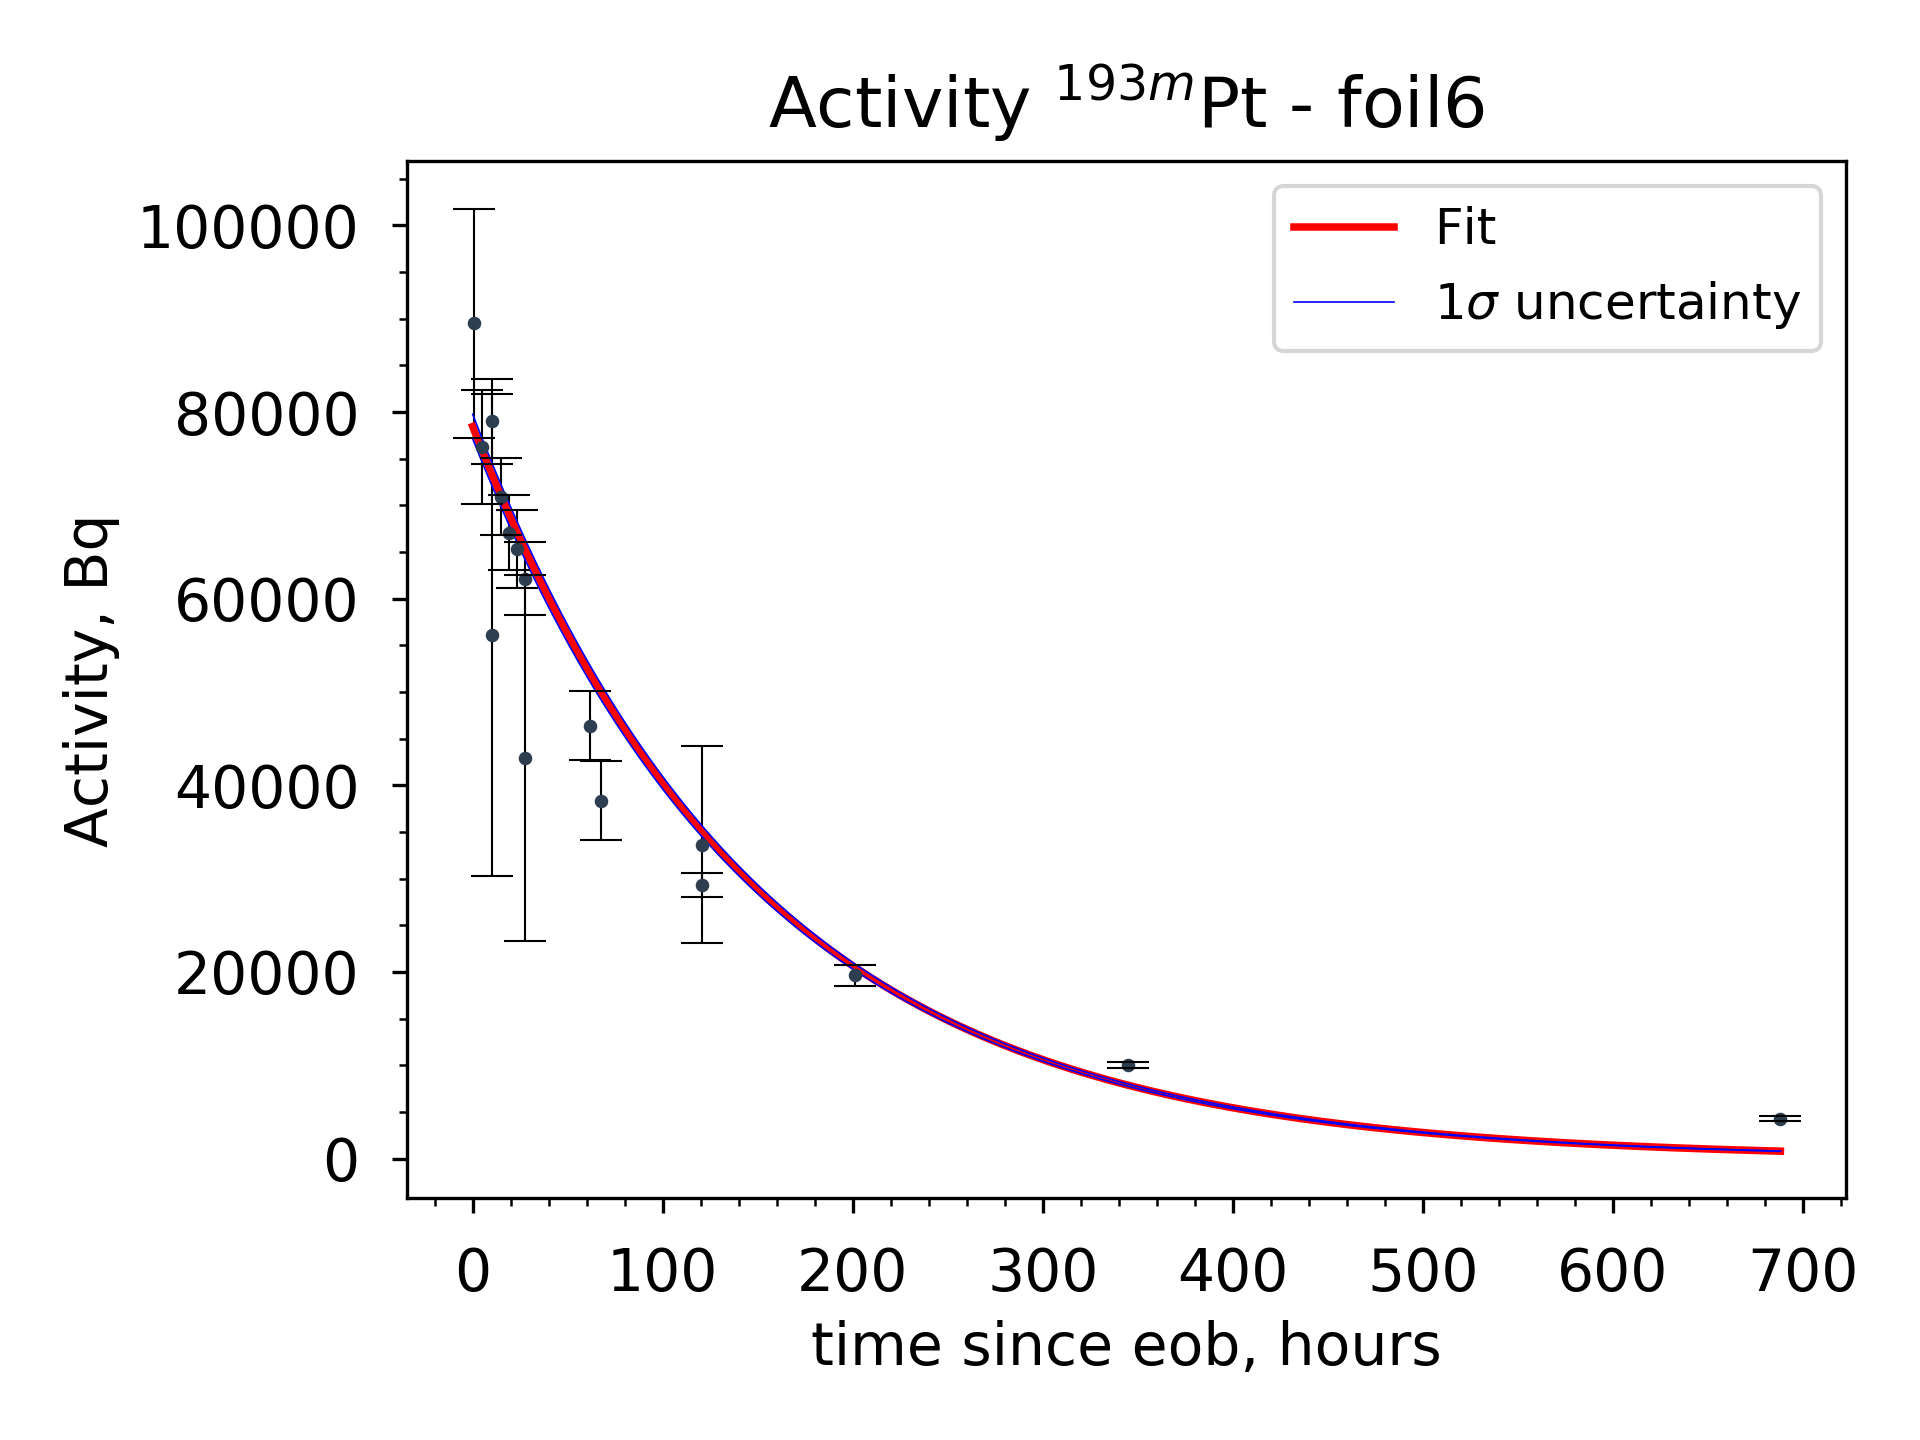
\includegraphics{Analysis/_activity_193mPt_677.png}
    \caption{An example of an activity curve using foil number 6 of $^{193m}$Pt with activities measured from the gamma ray spectroscopy using equation \ref{eq:activity_spectra}. The fitted curve is the single decay \textcolor{red}{Include two step decay also to give an example. } }  
    \label{fig:193mPt_activitycurve}
\end{figure}


\subsection{Beam Current}

The beam integrator gave a current of tube hitting the stack with 128.5 nA. However, due to the large energy degradation in the energy stack, there will be a certain spread in the beam, following scattering. This is also the first experiment which have used deuterium on a stack of targets, so beforehand, we did not know how much deuteron break-up would affect the current throughout the stack. Reactions from the copper, nickel and iron foils were used as monitor reactions to estimate the weighted average beam current which was used in the cross section calculation in equation \ref{eq:CS_ch3}. Well-known cross sections from IAEA were used\footnote{https://www-nds.iaea.org/medical/monitor_reactions.html. Need to add citation for each datapoint used.}; $^{\text{nat}}$Fe(d,x)$^{56}$Co, $^{\text{nat}}$Ni(d,x)$^{56,58}$Co and $^{\text{nat}}$Cu(d,x)$^{62,63,64}$Zn. \textcolor{red}{This method provides a more sensitive beam current calculation}. \\ 

\noindent 
In order to calculate the cross sections, we need an accurate measure of the beam current. Thus, with well-known cross sections from the monitor reactions, we can estimate the beam current: 

\begin{equation} \label{eq:BC_nodiff}
    \Phi = \frac{A_0}{N_T (1-e^{-\lambda \Delta t_\text{irr}})\sigma(\langle E\rangle)}
\end{equation}

\noindent 
In cross section experiments\footnote{based on special curriculum, p. 14}, the suggested value is a \textit{flux average cross section}, which implies that the cross section is dependent on the flux-weighted average beam energy. One single foil thus provides one cross section measurement, with the energy uncertainty only being dependent on the energy distribution in each foil. For thin targets, we assume a stopping power $dE/dx=0$ (a good approximation for targets which are less than 50 mg/cm$^2$ \textcolor{red}{citation?}), hence we can replace the cross section in equation \ref{eq:BC_nodiff} with the normalized 

\begin{equation}
    \sigma(\langle E \rangle) = \frac{\int \sigma(\langle E \rangle) \frac{d\phi(\langle E \rangle)}{dE}dE}{\int \frac{d\phi(\langle E \rangle)}{dE}dE}
\end{equation}

\noindent where $\sigma(\langle E \rangle)$ is the well-known monitor cross section from IAEA, $\phi/dE$ is the differential deuterium fluence.  Using the above expression, beamcurrent can be written on the form 

\begin{equation}
    \Phi(\langle E \rangle) = \frac{A_0}{N_T (1-e^{-\lambda \Delta t_\text{irr}})\frac{\int \sigma(\langle E \rangle) \frac{d\phi(\langle E \rangle)}{dE}dE}{\int \frac{d\phi(\langle E \rangle)}{dE}dE}}
\end{equation}

\noindent 
The energy degradation was measured using NPAT's (nuclear physics analysis tool) Ziegler simulation. The code is based on Ziegler stoppingpower formalism and Monte Carlo simulations \textcolor{red}{Write more about npat, and what type of formalism its based on}. However, the large challenges to the simulation is to assign the correct energy bins. Especially, in energy ranges where the cross section is very sensitive to changes (changes rapidly as a function of energy). Figure \ref{fig:Ir_Flux_Distr} shows the energy distribution in the foils, where the flux is along the y-axis. The further back in the stack the harder it is to model, hence the full width half maximum increases

Thus, a need of variance minimization was necessary to assure that the correct energy bins was assigned to the stack. 

\begin{figure}
    \centering
    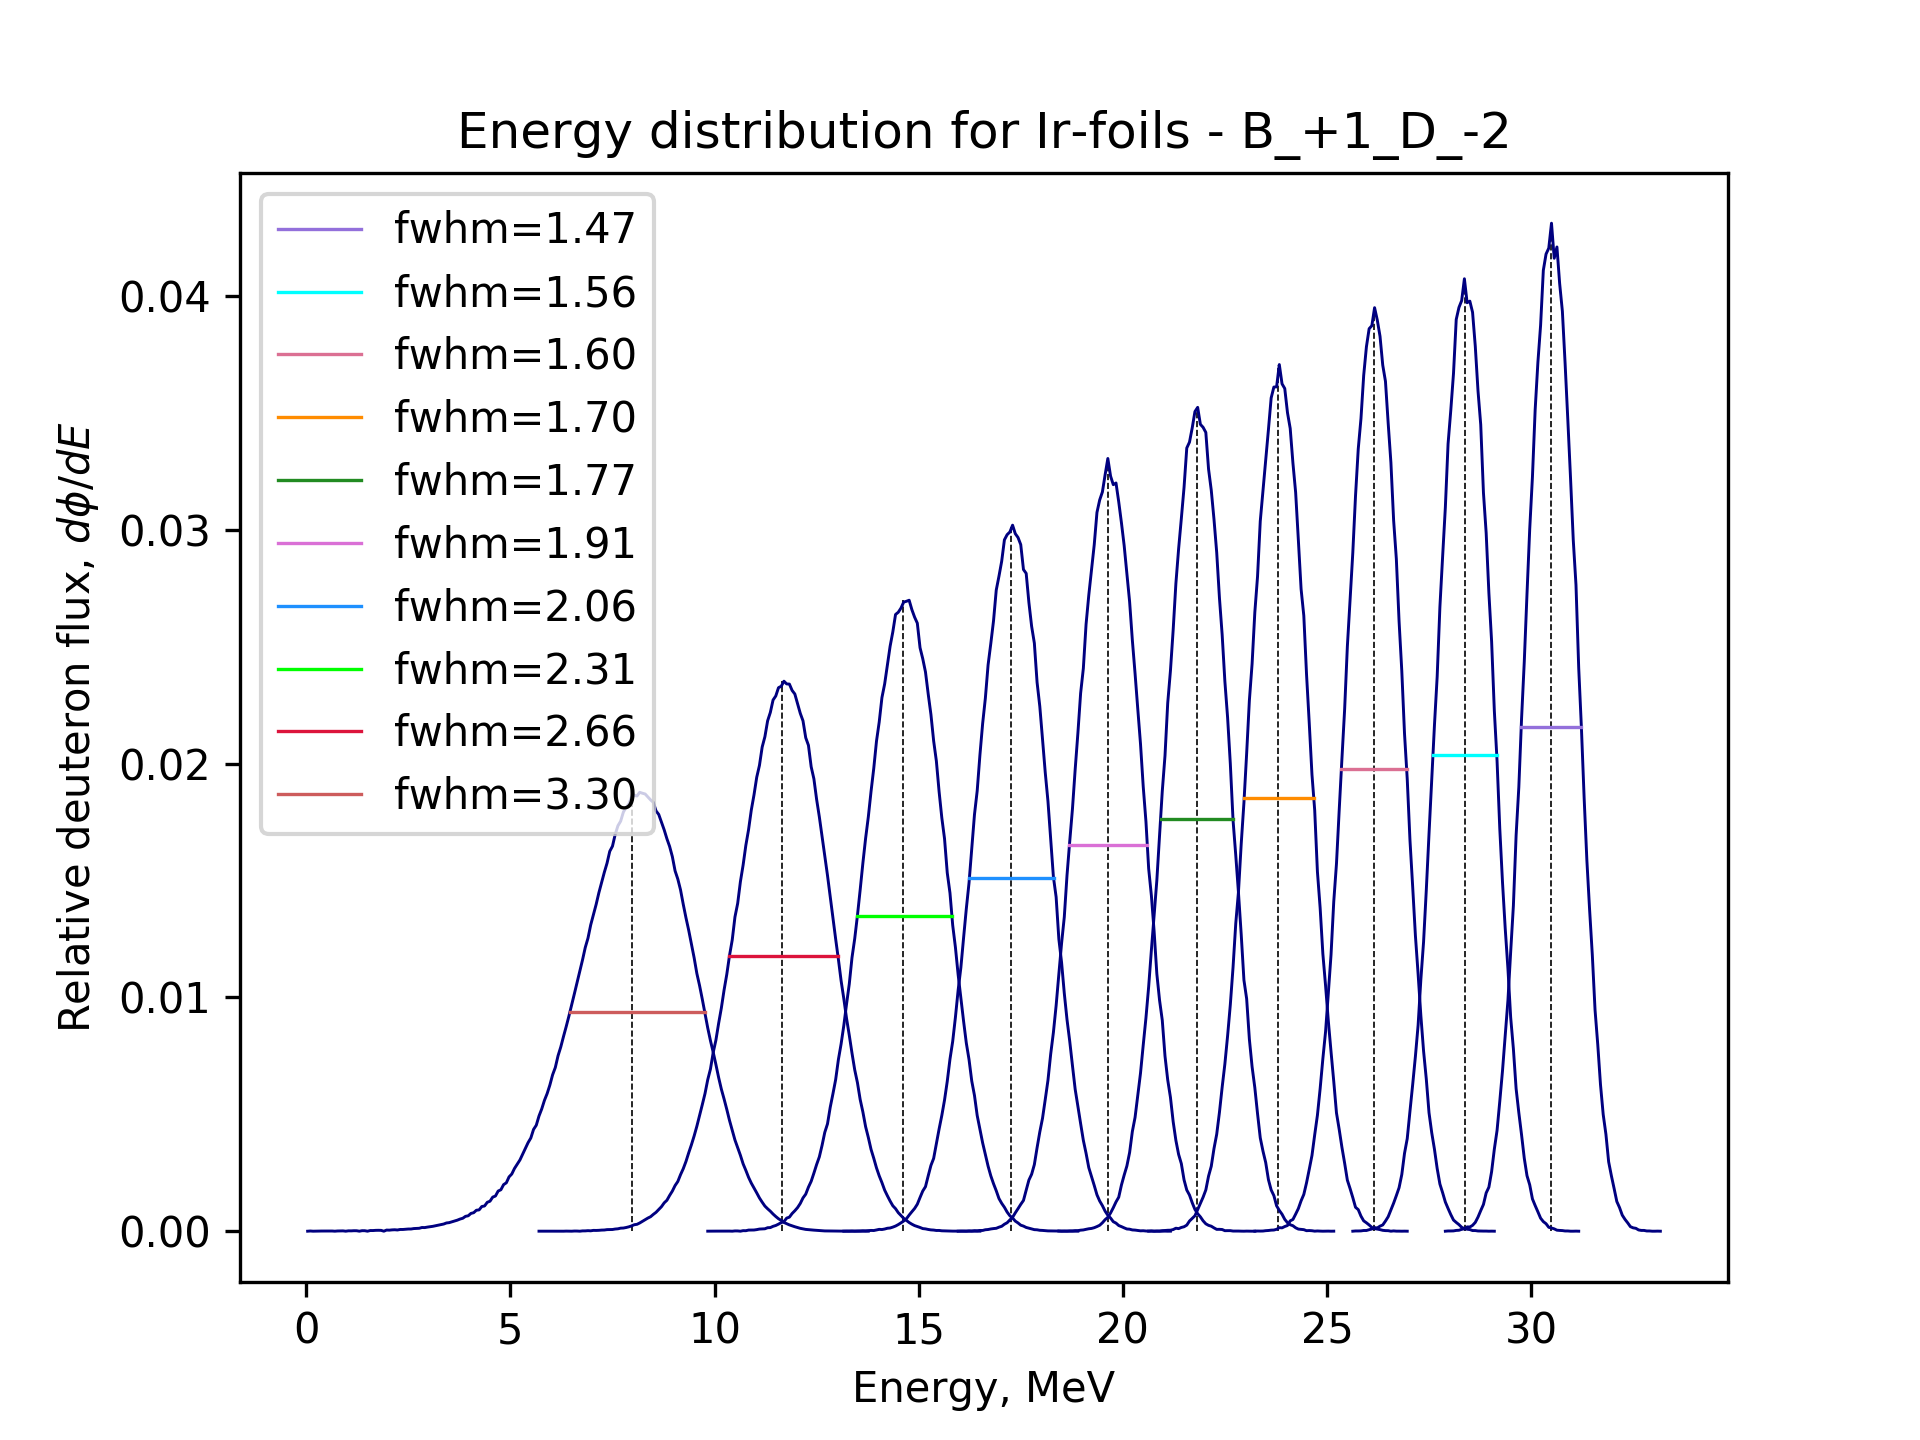
\includegraphics{Analysis/Ir_flux_distribution_B_+1_D_-2.png}
    \caption{The energy distribution of the iridium foils throughout the stack. \textcolor{red}{Should be very sure that it the beamcurrent in the end. } }
    \label{fig:Ir_Flux_Distr}
\end{figure}


\subsection{Variance minimization}
Ziegler files provides a set of energy and fluxes through the different foils. 
Did a areal density and beam energy increase and dicrease to see how it affected the current. Gives an energy distribution. Show figures.  \\

$\chi^2$ is an estimation of the goodness of fit which weight includes weight of error. The value is divided on the number of degrees of freedom (essensially the number of parameters minus 1. \textcolor{red}{why?})
\begin{equation} \label{eq:chi_squared}
    \chi^2 = \sum_{i}^n \Big(\frac{ y_i - \overline{y}}{ \sigma_i} \Big)^2 
\end{equation}

\noindent 
The idea was to get an estimation of the values of $\chi^2$ over the different compartments (one compartment is one set of foils, for instance Ni01, Ir01, Fe01 and Cu01). Compartment 3, 6 and 9 was investigated to get an idea of the scaling parameter that gave lowest values. If we cared about the $\chi^2$ values at high energies (early in the stack), the currents tend to be bad in the back of the stack, due to scattering at compartment 3 being low. However, in compartment 3, we had 7 independent measurements of beam current which gave more data. In compartment 9, a lot of the currents were low due to most reactions being at the energy threshold. Hence compartment 6 was used, which had 5 measurements (61Cu, 56,58Co, 63,65Zn). 62Zn was below threshold, and iron did not have any foil in compartment 6. The compartment can be seen in figure \ref{fig:varmin_comp6}. 

\begin{figure}
    \centering
    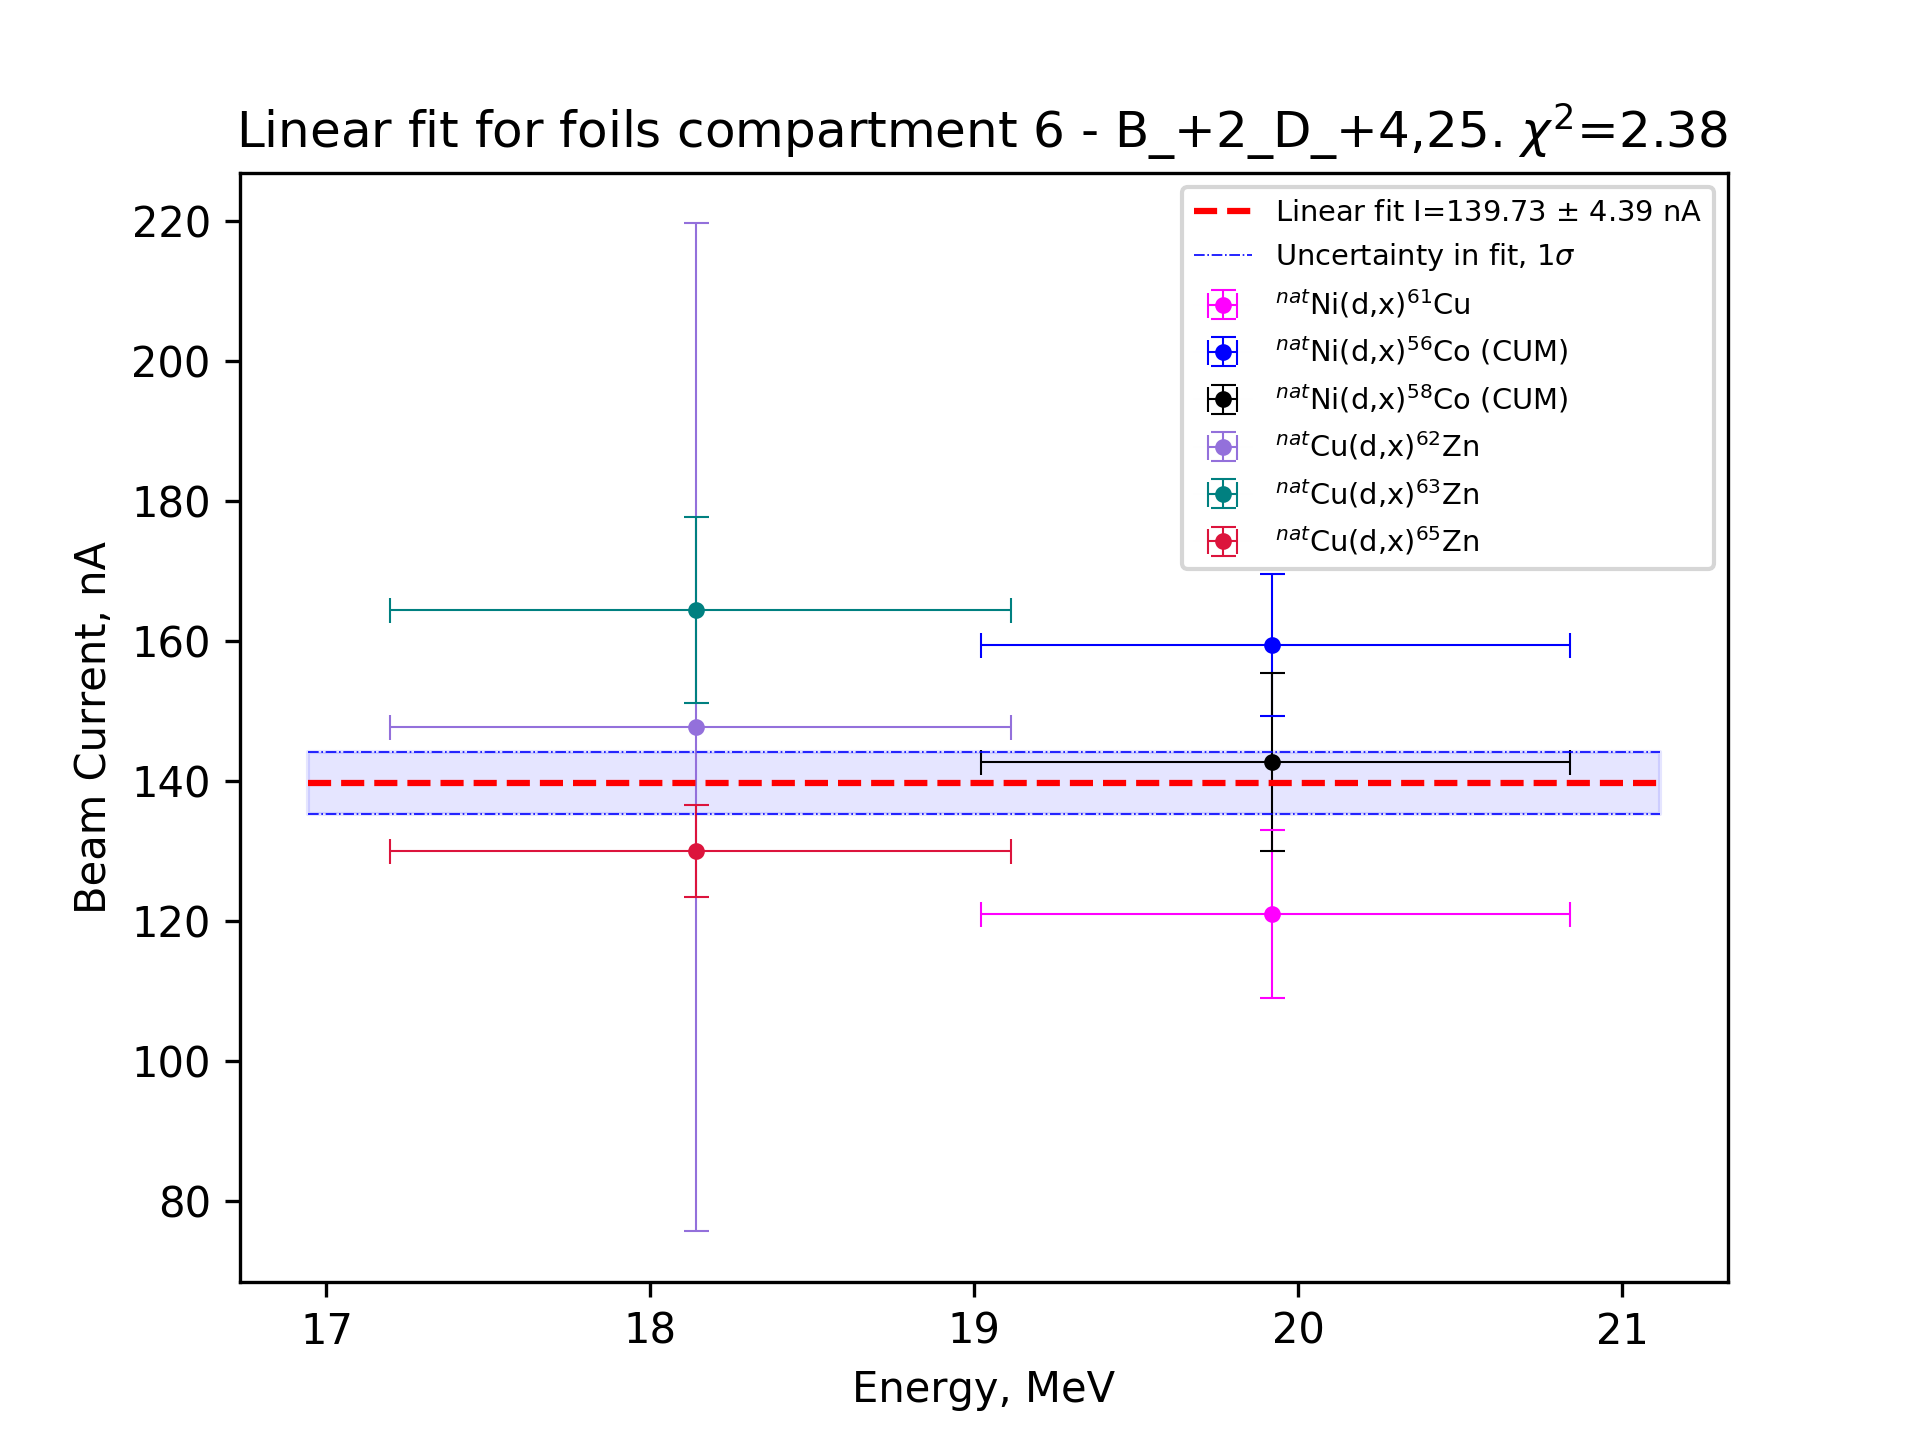
\includegraphics{Analysis/minimization_6_B_+2_D_+4,25.png}
    \caption{Variance minimization in compartment 6.}
    \label{fig:varmin_comp6}
\end{figure}

Assuming constant beam current in one compartment. Hence we can have a linear fit between the beam current measurements. With no current degradation, $y=mx+b$, m=0, b is initial guess of 128.5 nA. 

\begin{figure}%
    \centering
    \subfloat[Before variance minimization]{{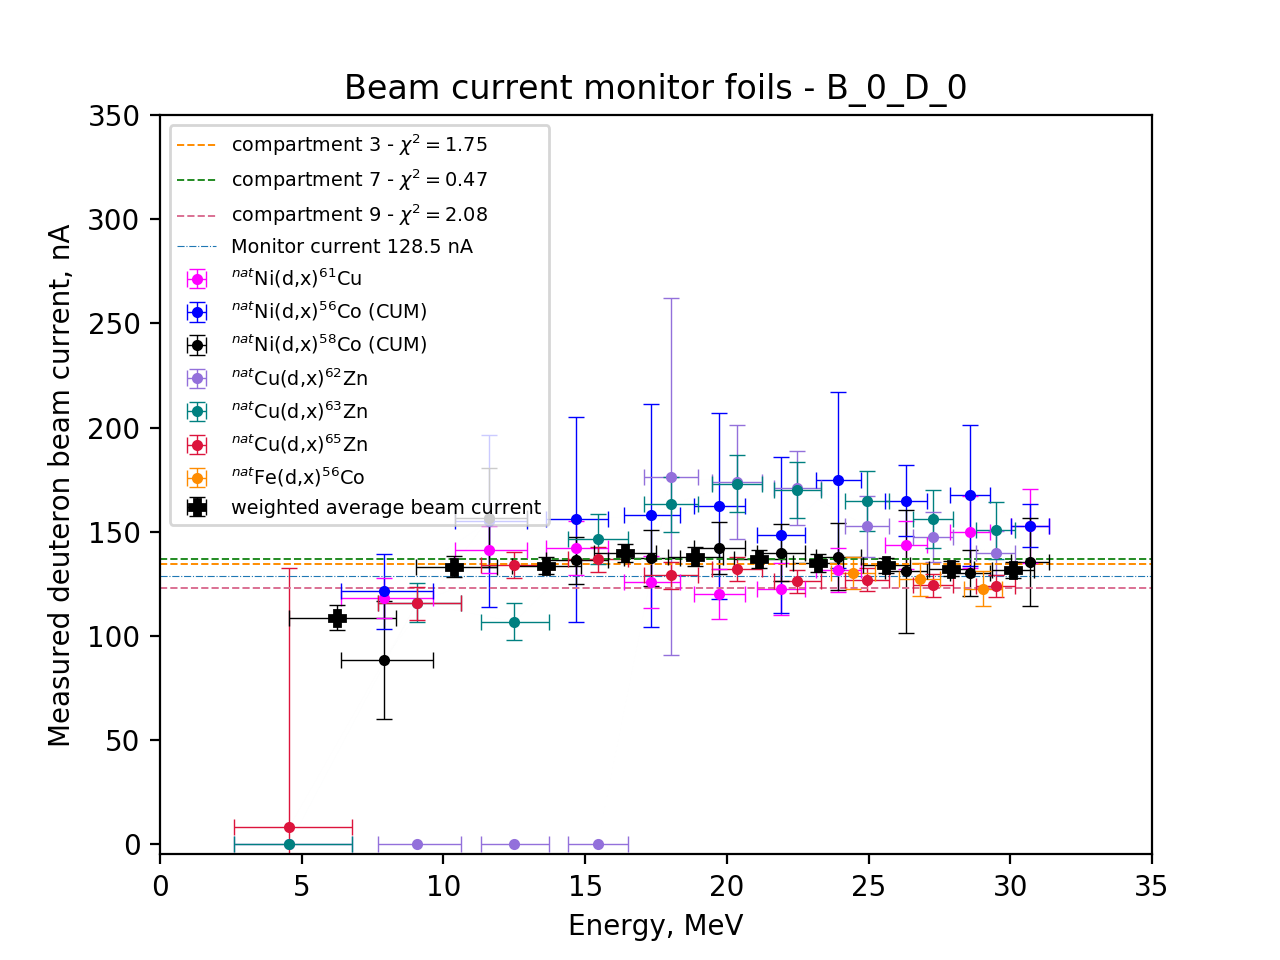
\includegraphics[width=8cm]{Analysis/B_0_D_0.png} }}%
    \quad
    \subfloat[After variance minimization]{{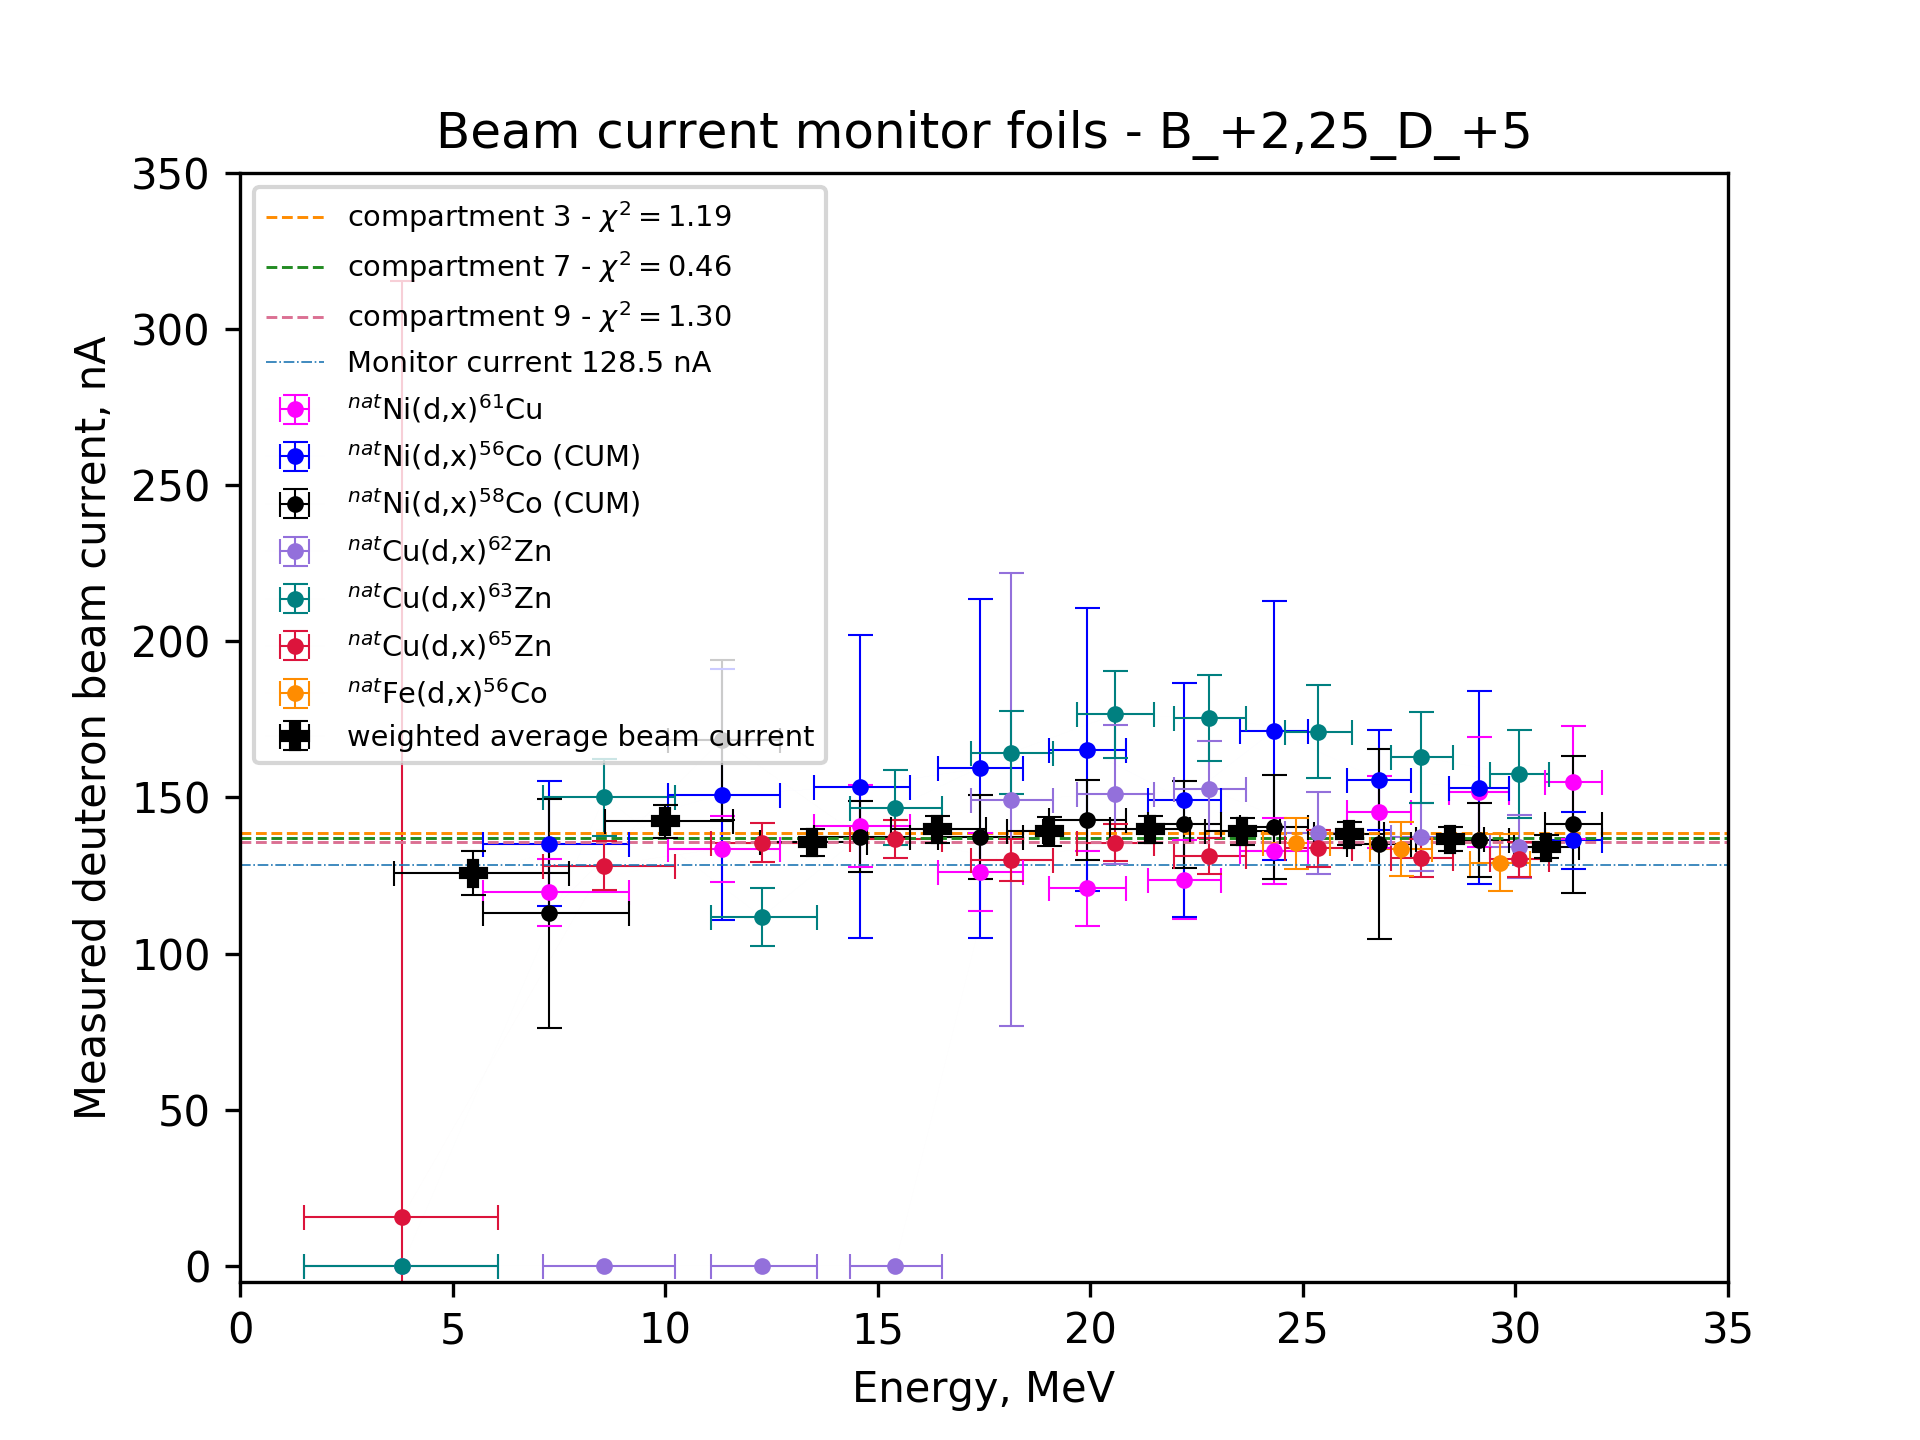
\includegraphics[width=8cm]{Analysis/comp_compared_B_+2,25_D_+5.png} }}%
    \caption{Before, the current in the back of the stack is tending to be lower. The $\chi^2$ in the different compartments also tend to be higher. After variance minimization, the values for $\chi^2$ are smaller and the estimated current in each compartment agrees more with each other. We do not expect much of current degradation.}%
    \label{fig:varmin_beamcurrent}%
\end{figure}


\subsubsection{The weighted averaged beam current, along with uncertainties}

Need to write statistical part first, about covariance matrix. 


Testing: the weighted average beam current for each target foil was used, to estimate the cross section. 

\begin{figure}%
    \centering
    \subfloat[]{{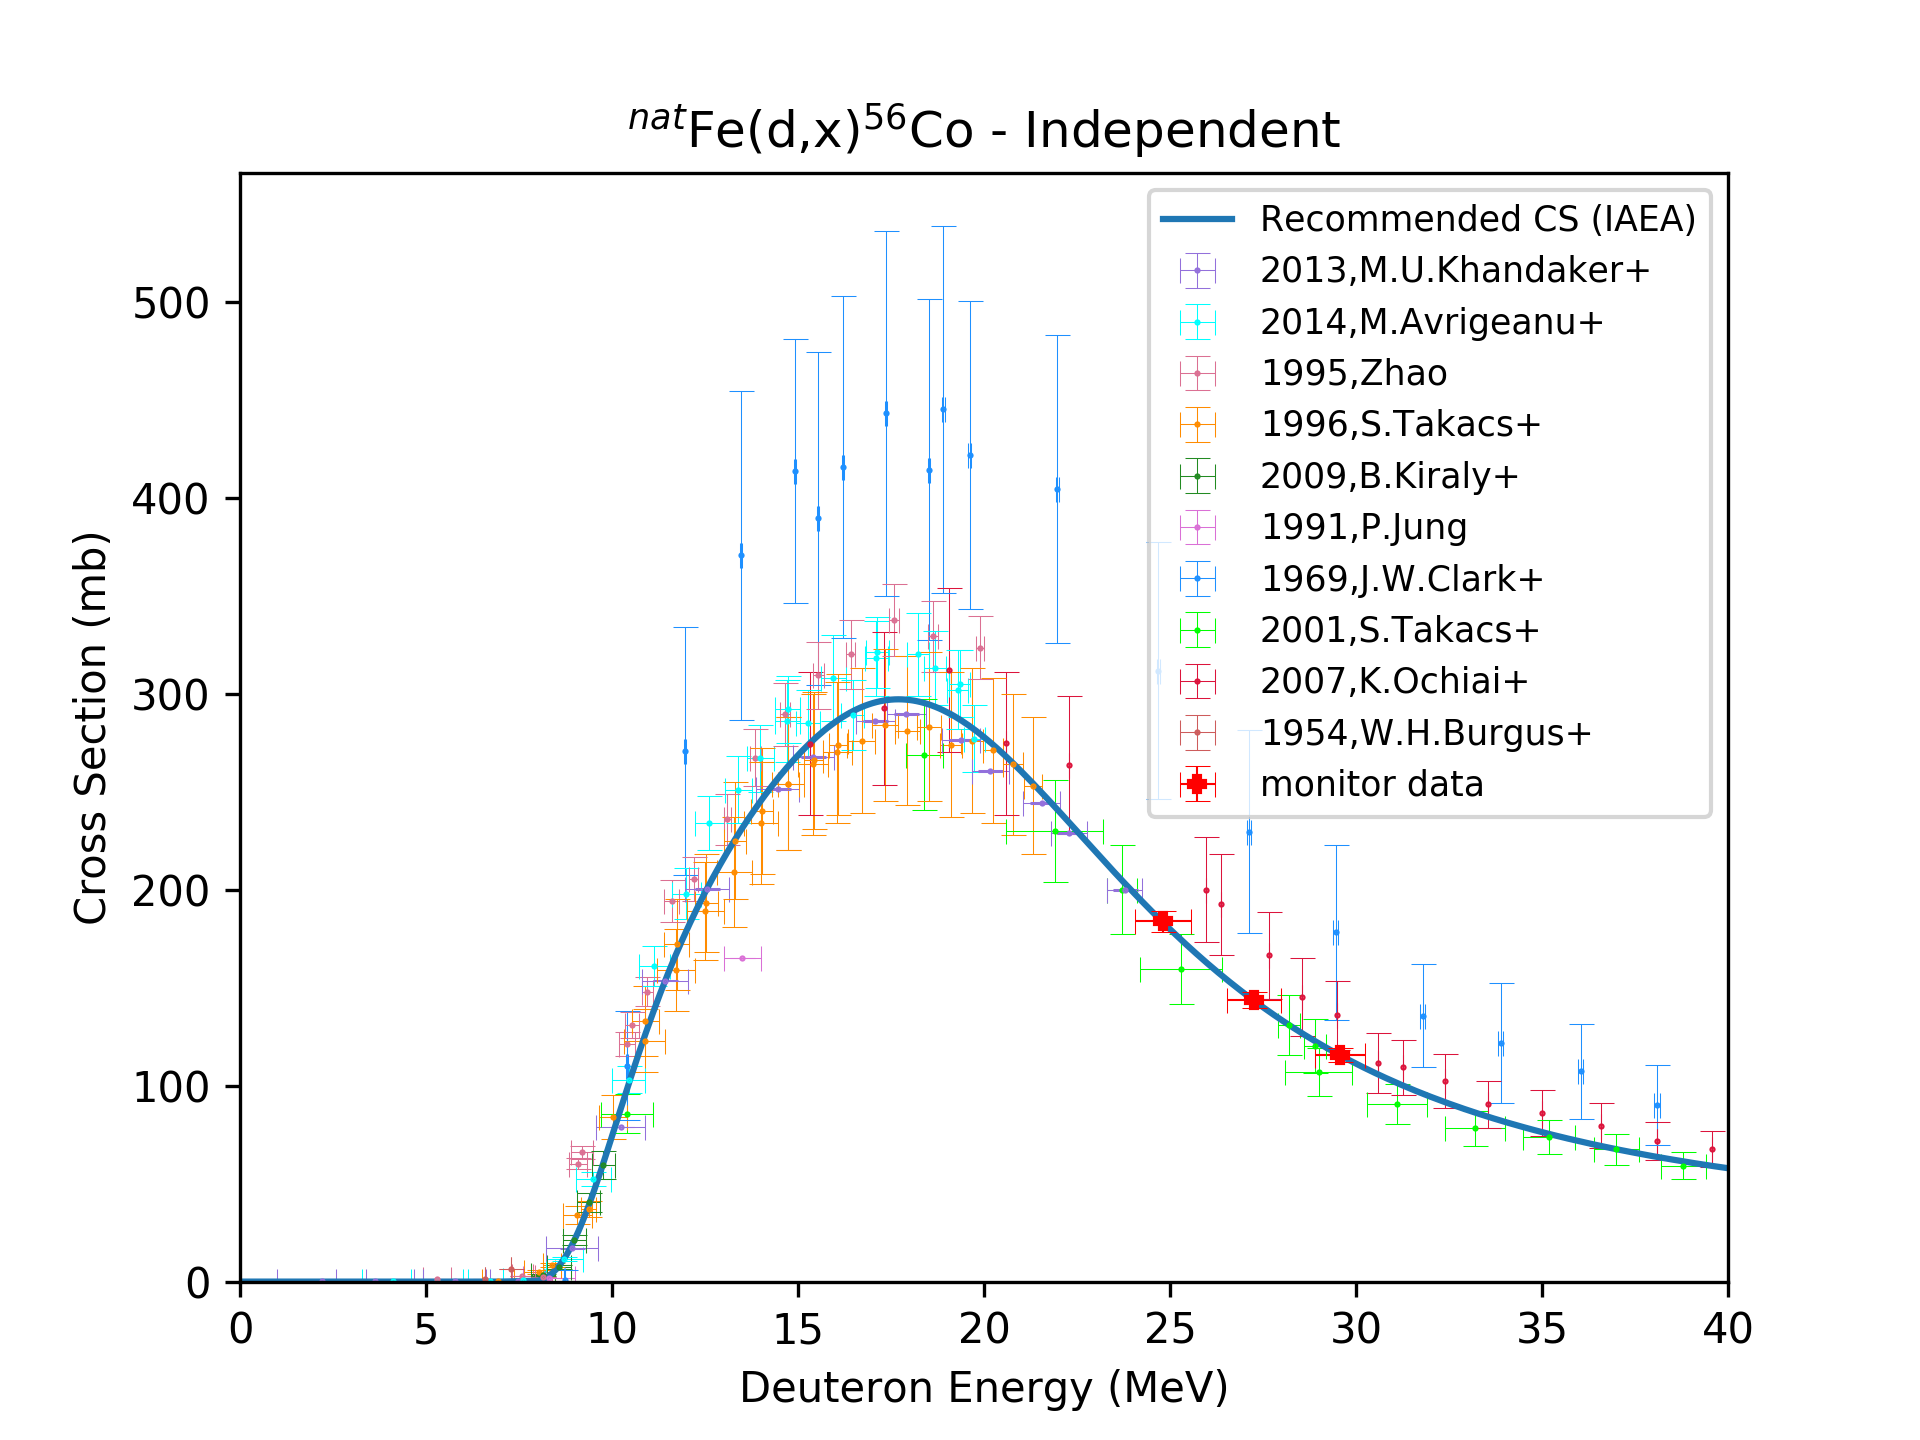
\includegraphics[width=5cm]{Analysis/Fe_56Co.png} }}%
    \quad
    \subfloat[]{{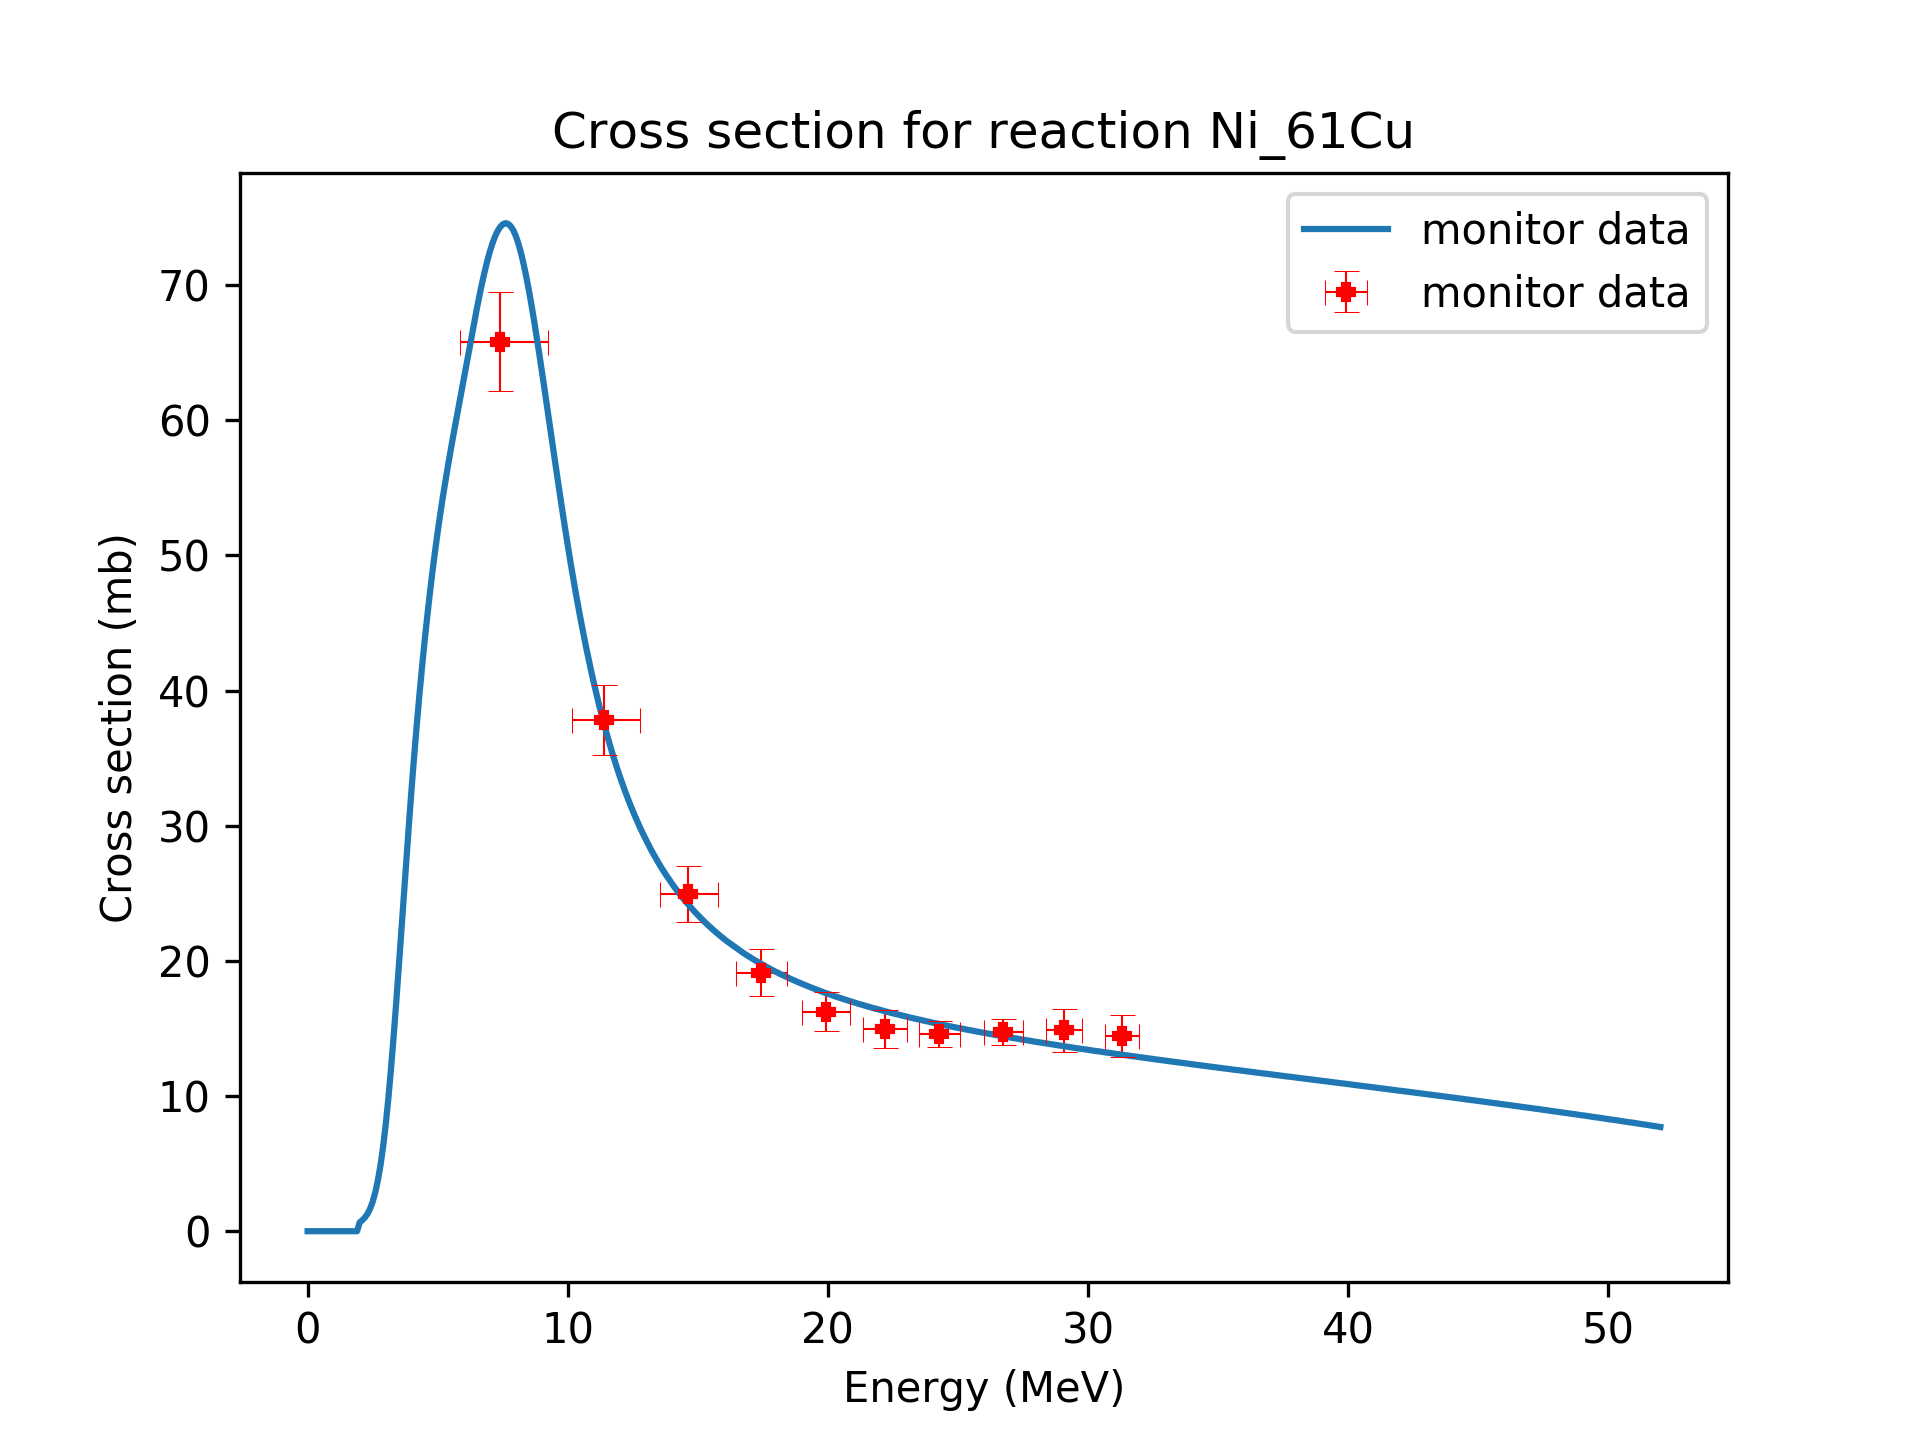
\includegraphics[width=5cm]{Analysis/Ni_61Cu.png} }}%
    \subfloat[]{{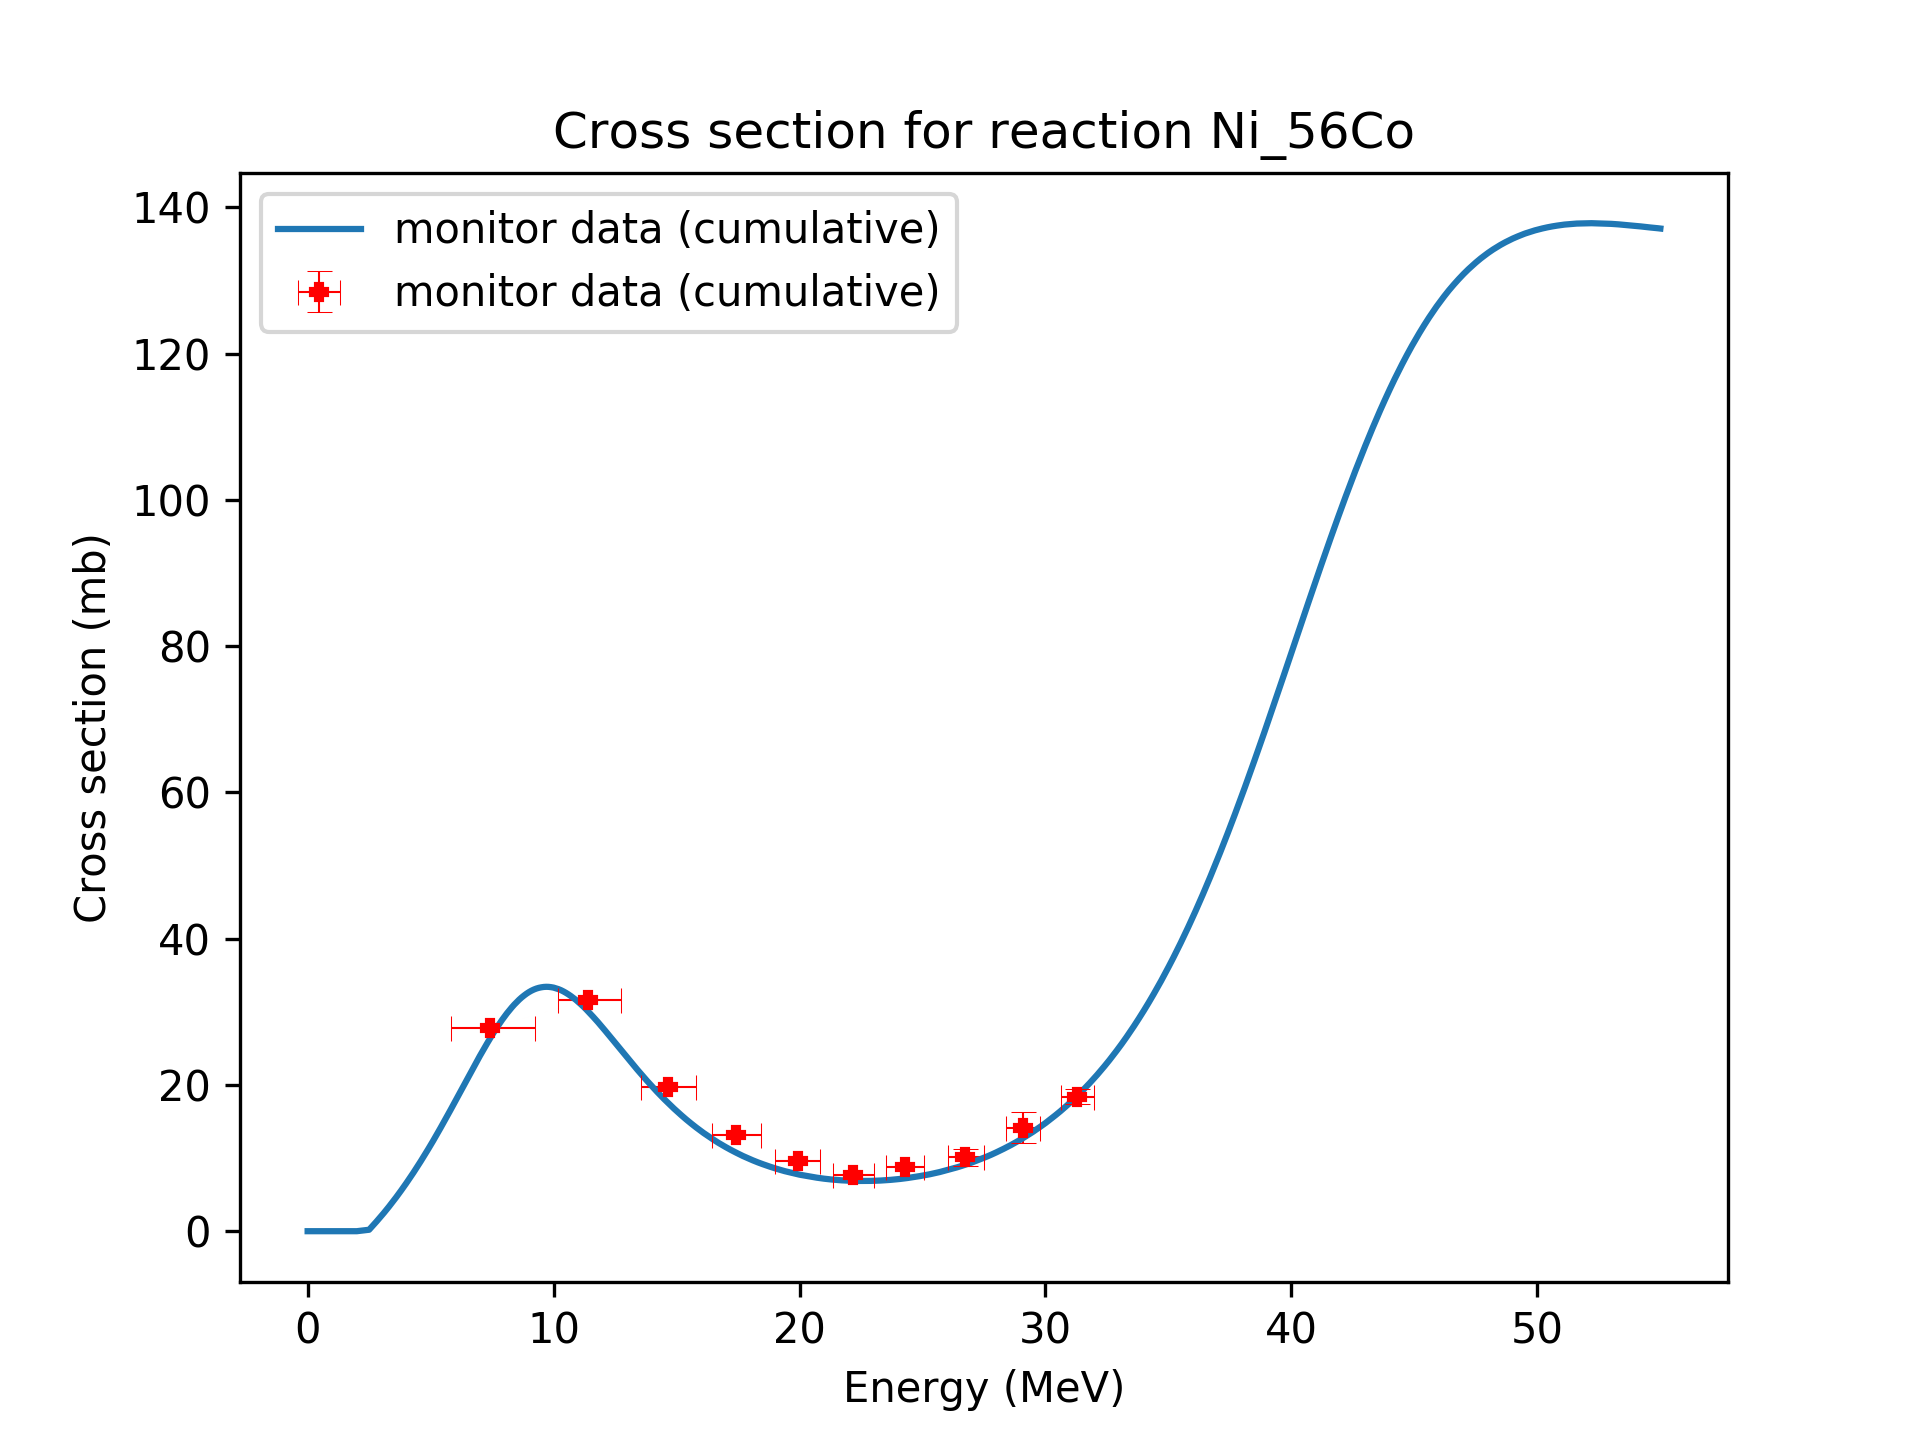
\includegraphics[width=5cm]{Analysis/Ni_56Co.png} }}%
    \quad
    \subfloat[]{{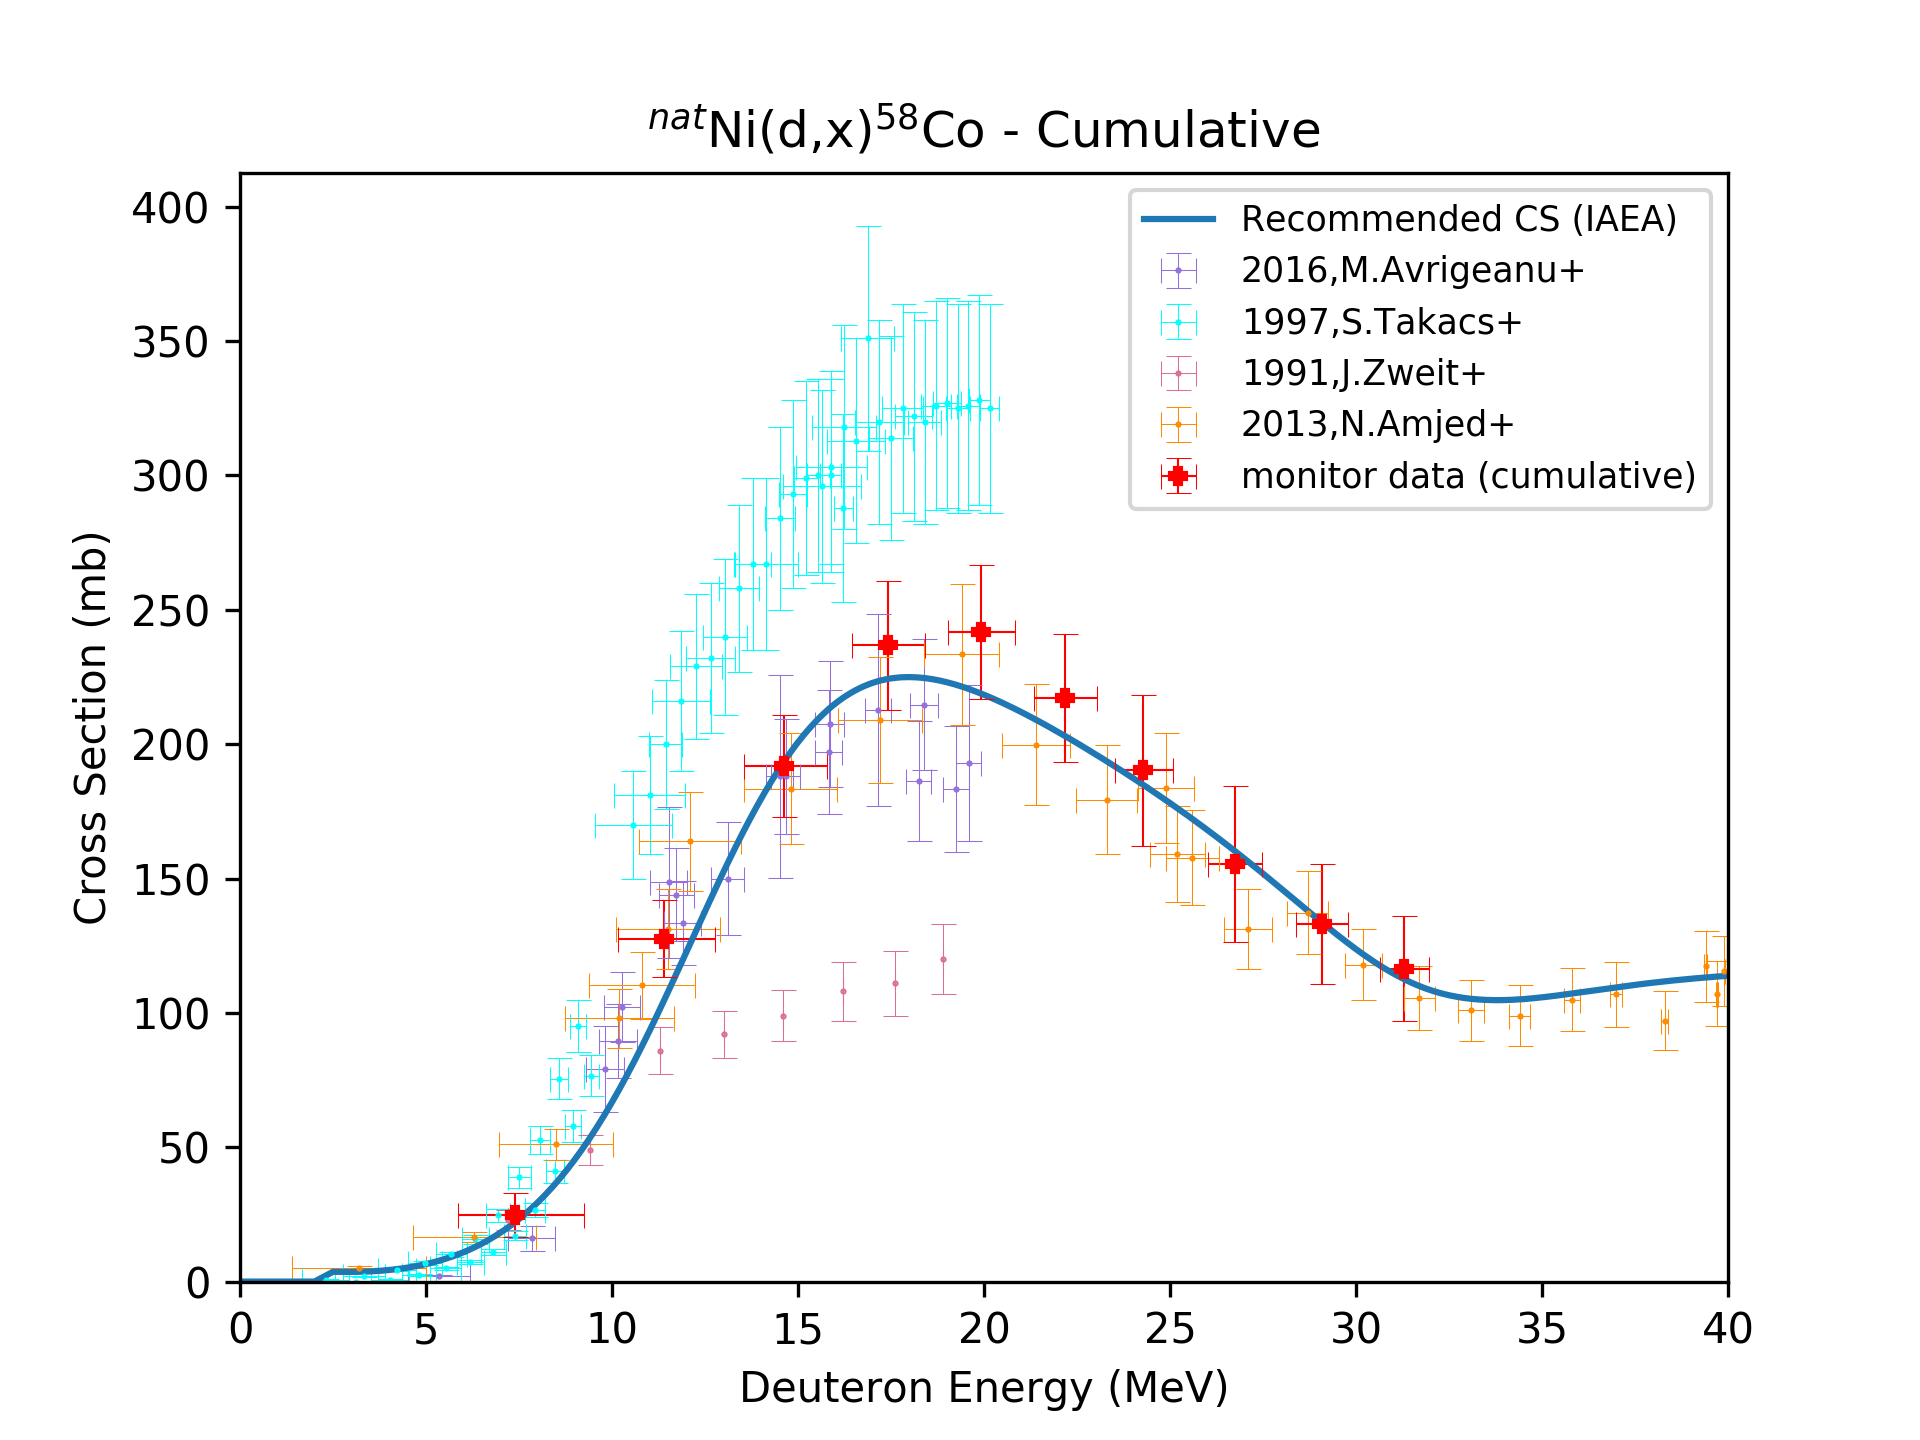
\includegraphics[width=5cm]{Analysis/Ni_58Co.png} }}%
    \quad
    \subfloat[caption]{{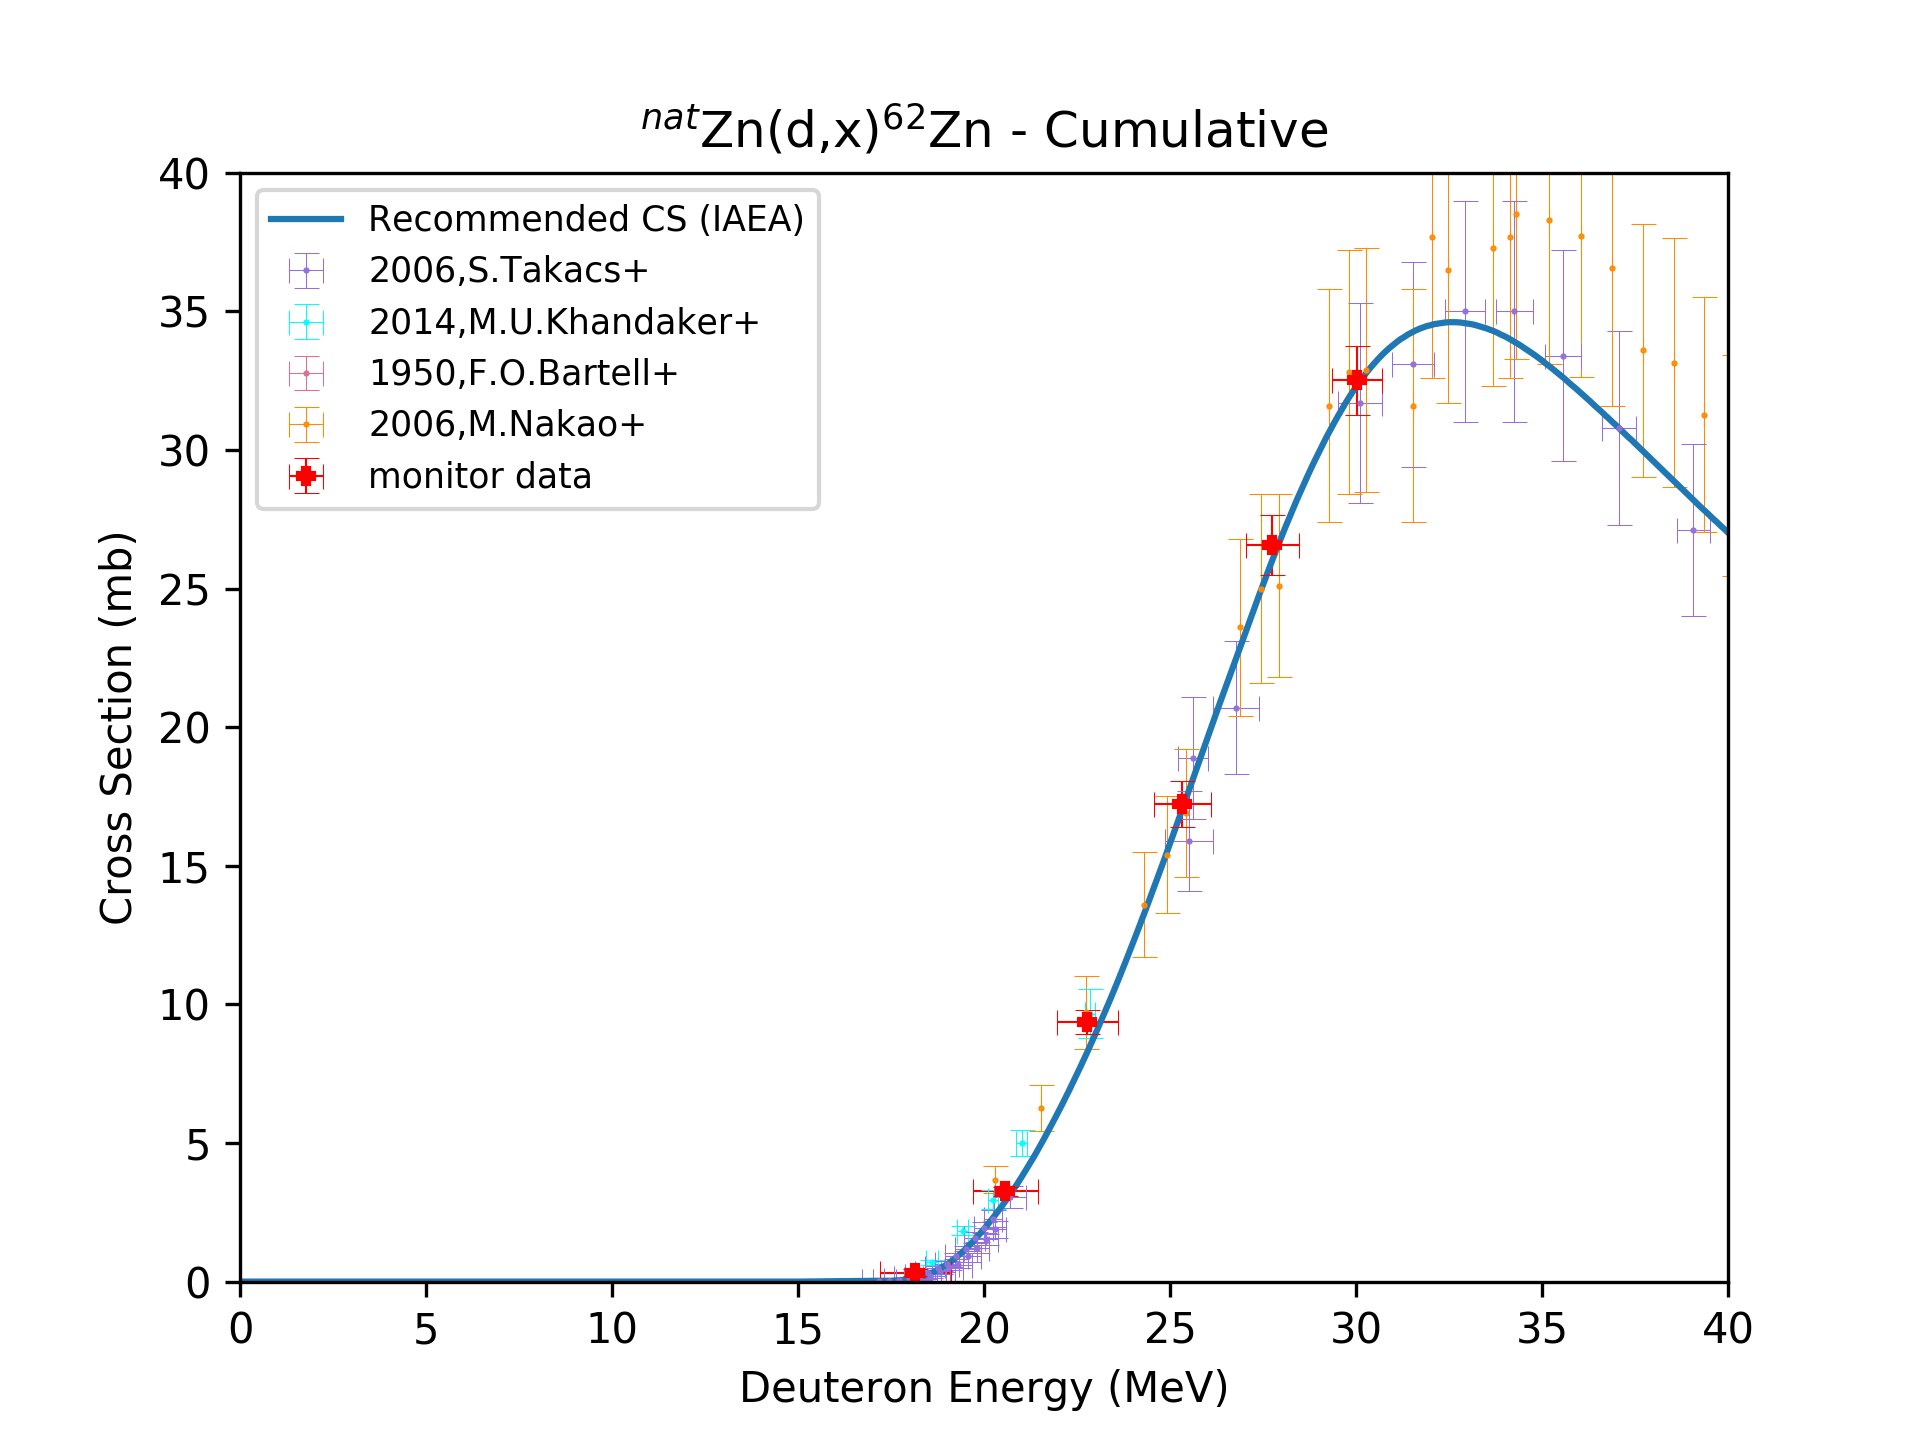
\includegraphics[width=5cm]{Analysis/Cu_62Zn.png} }}%
    \quad
    \subfloat[]{{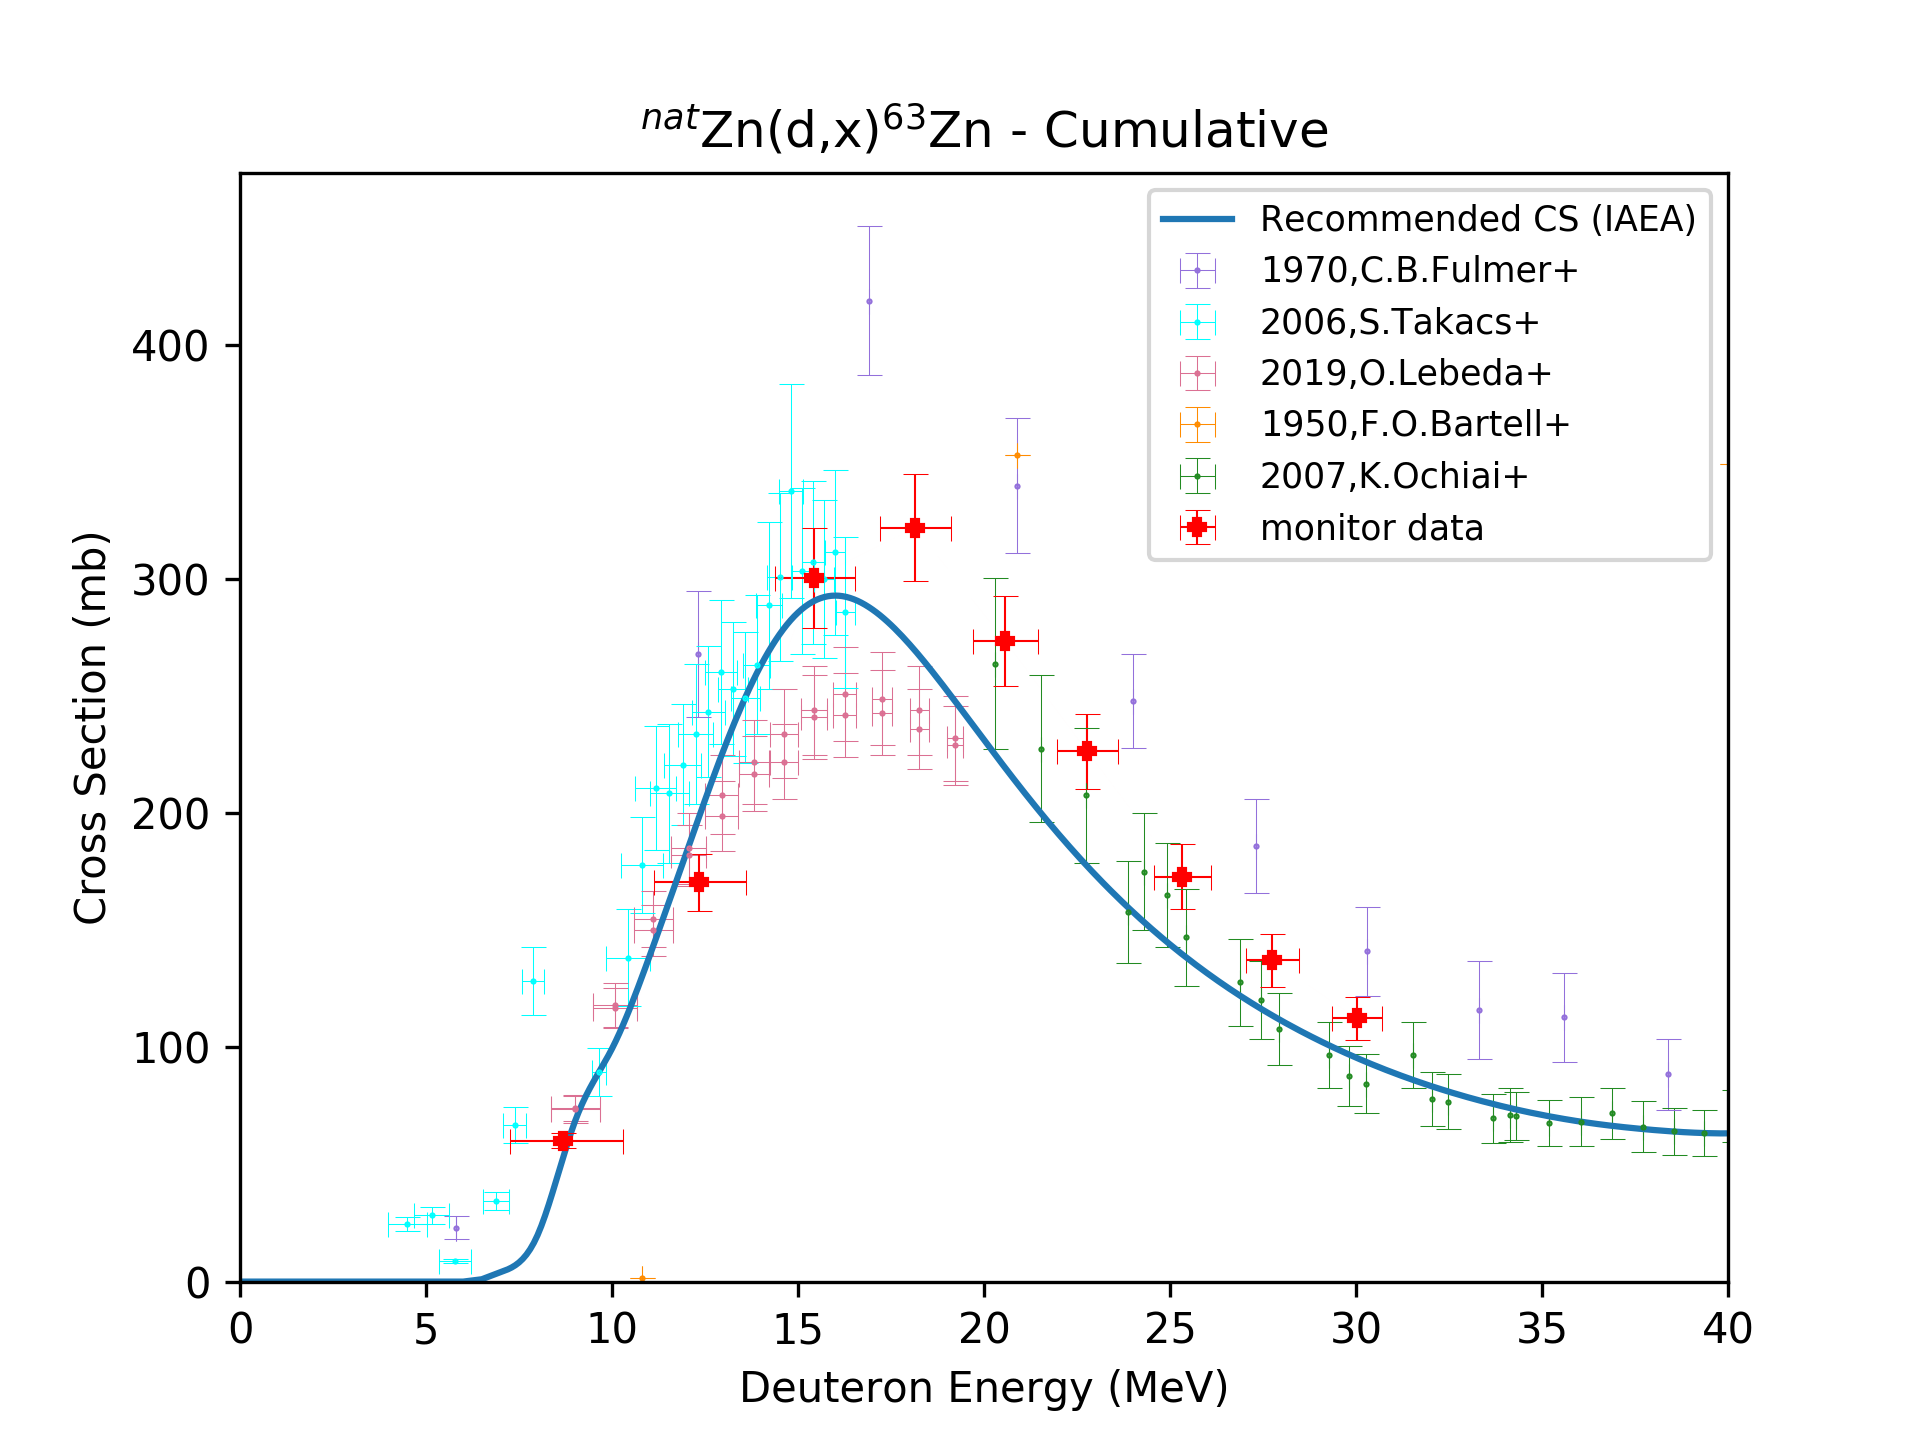
\includegraphics[width=5cm]{Analysis/Cu_63Zn.png} }}%
    \quad
    \subfloat[]{{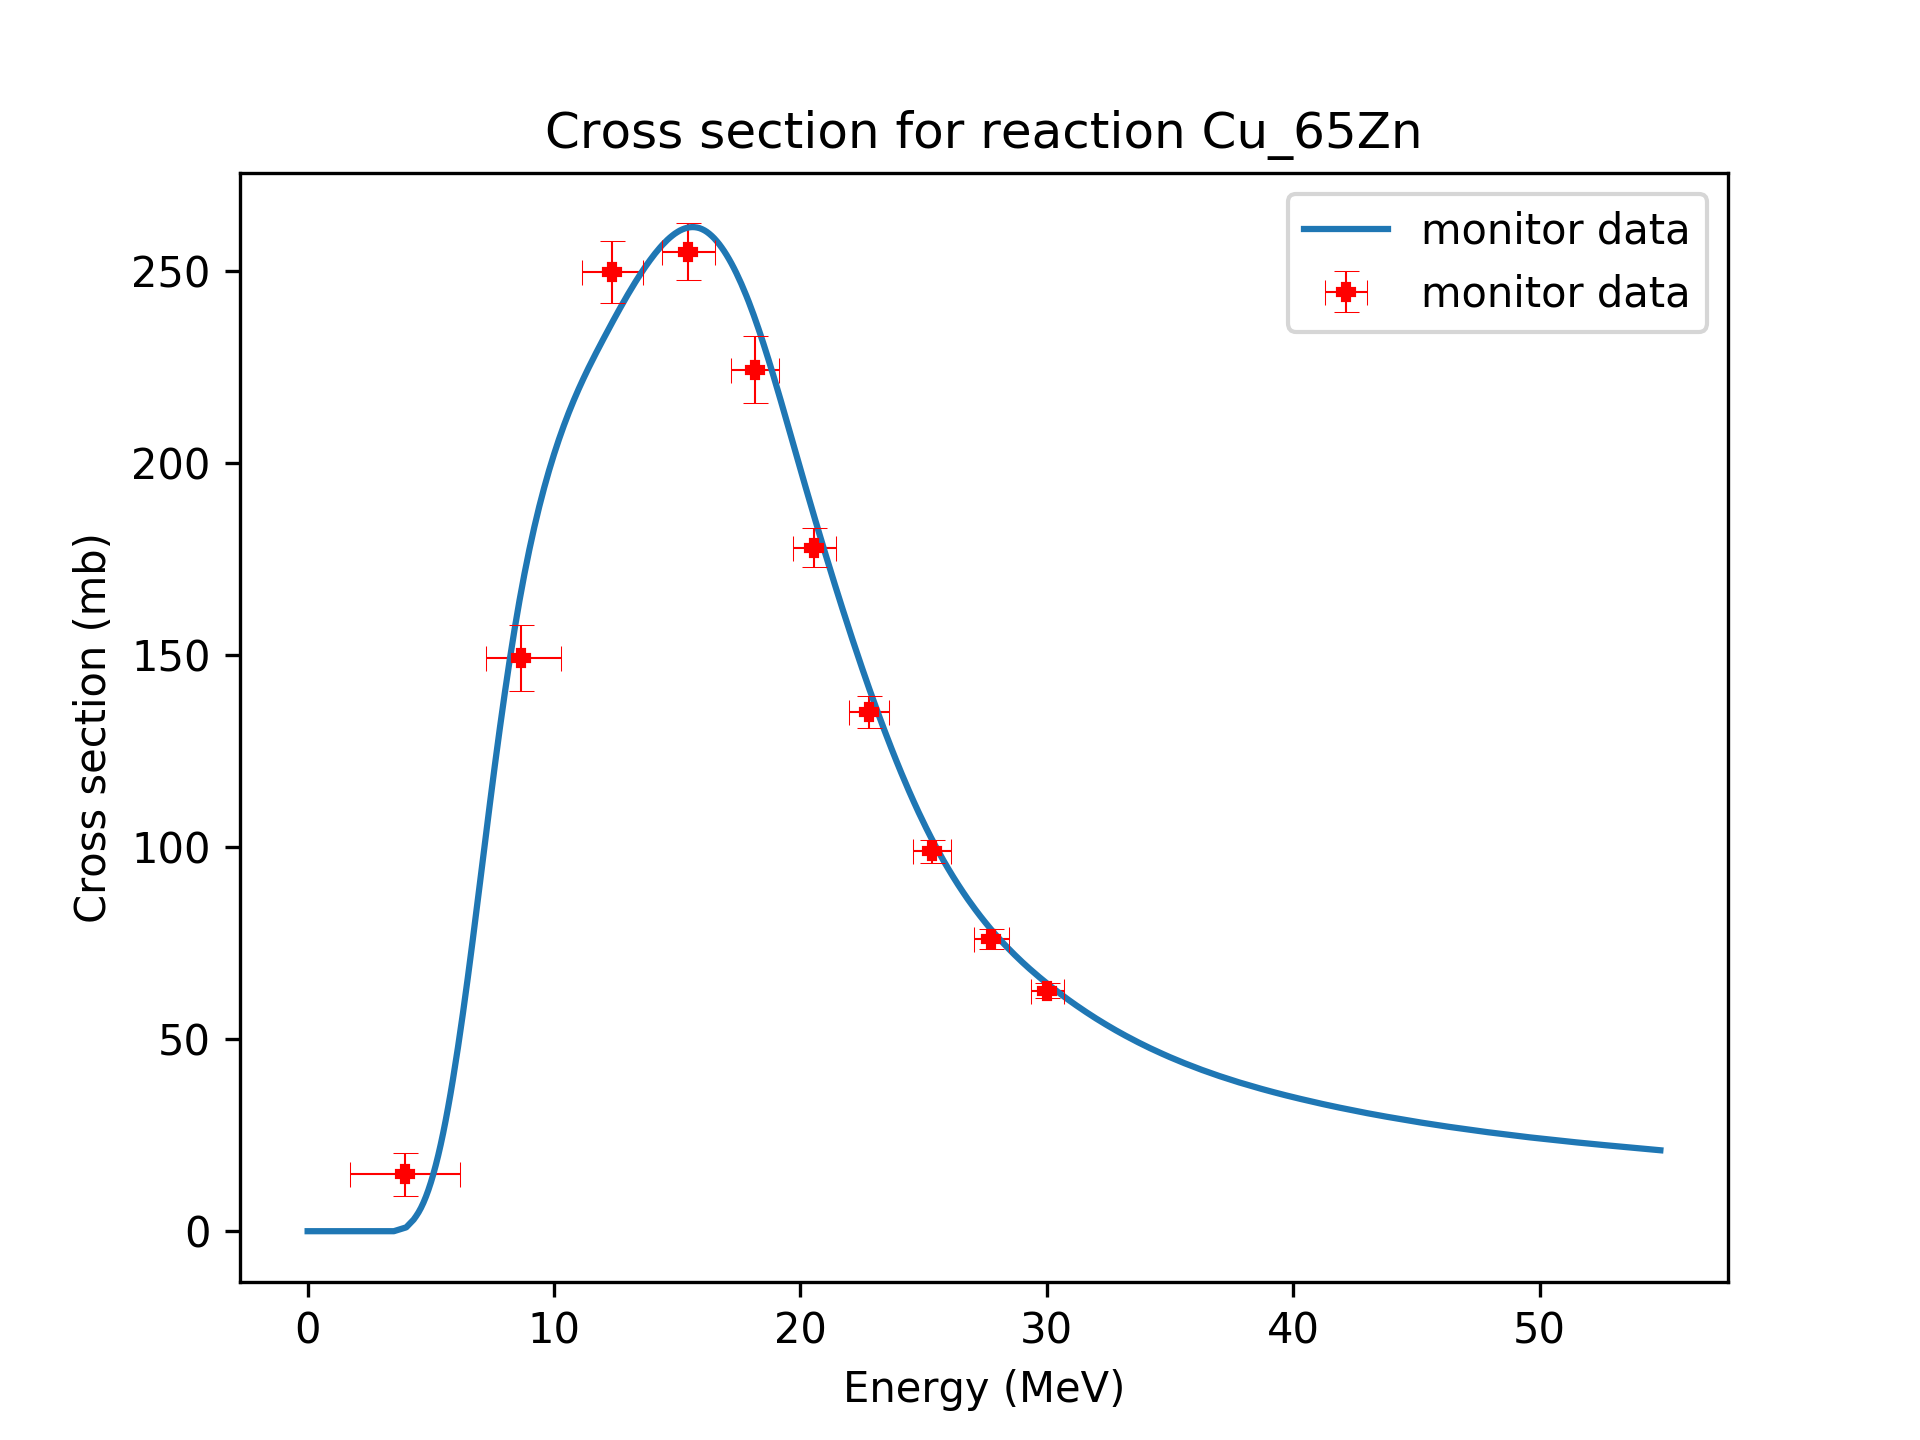
\includegraphics[width=5cm]{Analysis/Cu_65Zn.png} }}%
    \quad
    \caption{Figure shows the estimation of monitor cross section using the calculated beam current. It is compared along with the monitor data.  }%
    \label{fig:monitor_BC}%
\end{figure}



\subsection{Production Cross sections}

Once the weighted average beam current was estimated, the cross sections were estimated using equation \ref{eq:CS_ch3}. For decay chains, the first observed element was reported as cumulative, unless it was the first entry. If there was independent measurements of the daughter products, they were reported as independent and cumulative along with the parent. 






